\documentclass[13pt,a4paper]{report}
\usepackage[utf8x]{inputenc}
\usepackage[english=nohyphenation]{hyphsubst}
\usepackage[english]{babel}
\usepackage{titlesec, blindtext, color}
\usepackage[table,xcdraw,dvipsnames]{xcolor}

\title{KL Document}
\author{Cong Le Ba}

\newcommand{\mychapter}[2]{
    \setcounter{chapter}{#1}
    \setcounter{section}{0}
    \chapter*{#2}
    \addcontentsline{toc}{chapter}{#2}
    }

\definecolor{gray75}{gray}{0.75}
\newcommand{\hsp}{\hspace{15pt}}
\titleformat{\chapter}[hang]{\small\bfseries}{\thechapter\hsp\textcolor{gray75}{|}\hsp}{0pt}{\Huge\bfseries}
\usepackage[left=3cm,right=2cm,top=2.5cm,bottom=3cm]{geometry}
\setlength{\parindent}{1cm}
\usepackage{indentfirst}    
\setlength{\parskip}{6pt}
\usepackage{sectsty}
\chapterfont{\centering}
\renewcommand{\baselinestretch}{1.3} %format distance between lines
\usepackage{xcolor}
\usepackage[unicode]{hyperref}
\hypersetup{
colorlinks = false,
linkbordercolor = {white}
}
\usepackage{graphicx}
\usepackage{lmodern}
\usepackage[font=small,labelfont=bf]{caption} % Required for specifying captions to tables and figures
\usepackage{bm}
\usepackage[para]{footmisc}
\usepackage{amsfonts}
\usepackage{afterpage}
\usepackage{float}
\usepackage{tikz}
\usepackage{pdfpages}
\usepackage{xspace}
\usepackage{dirtree}

\usetikzlibrary{calc}
\usepackage{frontespizio}
% \usepackage[perpage]{footmisc}
\usepackage{perpage}
\MakePerPage{footnote}
\usepackage{longtable}
\usepackage{sectsty}
\usepackage{ragged2e}
% format titile chapter section ...
\titleformat{\chapter}[display]
{\large}
{
	\large\MakeUppercase{\chaptertitlename}~\thechapter}
{1pc}
{\titlerule\huge}

\titleformat*{\section}{\normalfont \Large}
\titleformat*{\subsection}{\normalfont \large}

% code
\usepackage{listings}

\definecolor{codegreen}{rgb}{0,0.6,0}
\definecolor{codegray}{rgb}{0.5,0.5,0.5}
\definecolor{codepurple}{rgb}{0.58,0,0.82}
\definecolor{backcolour}{rgb}{0.95,0.95,0.92}

\lstdefinestyle{mystyle}{
    backgroundcolor=\color{backcolour},   
    commentstyle=\color{codegreen},
    keywordstyle=\color{magenta},
    numberstyle=\tiny\color{codegray},
    stringstyle=\color{codepurple},
    basicstyle=\small,
    breakatwhitespace=false,         
    breaklines=true,                 
    captionpos=b,                    
    keepspaces=true,                 
    numbers=left,                    
    numbersep=5pt,                  
    showspaces=false,                
    showstringspaces=false,
    showtabs=false,                  
    tabsize=2,
  keywords={!in, !is, abstract, actual, annotation, as, as?, break, by, catch, class, companion, const, constructor, continue, crossinline, data, delegate, do, dynamic, else, enum, expect, external, false, field, file, final, finally, for, fun, get, if, import, in, infix, init, inline, inner, interface, internal, is, lateinit, noinline, null, object, open, operator, out, override, package, param, private, property, protected, public, receiveris, reified, return, return@, sealed, set, setparam, super, suspend, tailrec, this, throw, true, try, typealias, typeof, val, var, vararg, when, where, while},
  keywordstyle={\color{NavyBlue}\bfseries},
  emph={filter, first, firstOrNull, forEach, lazy, map, mapNotNull, println},
  emphstyle={\color{OrangeRed}},
  comment=[l]{//},
  commentstyle={\color{gray}\ttfamily},
}

\lstset{style=mystyle}


\lstdefinelanguage{ABC}{
  comment=[l]{//},
  commentstyle={\color{gray}\ttfamily},
  emph={filter, first, firstOrNull, forEach, lazy, map, mapNotNull, println},
  emphstyle={\color{OrangeRed}},
  identifierstyle=\color{black},
  keywords={!in, !is, abstract, actual, annotation, as, as?, break, by, catch, class, companion, const, constructor, continue, crossinline, data, delegate, do, dynamic, else, enum, expect, external, false, field, file, final, finally, for, fun, get, if, import, in, infix, init, inline, inner, interface, internal, is, lateinit, noinline, null, object, open, operator, out, override, package, param, private, property, protected, public, receiveris, reified, return, return@, sealed, set, setparam, super, suspend, tailrec, this, throw, true, try, typealias, typeof, val, var, vararg, when, where, while},
  keywordstyle={\color{NavyBlue}\bfseries},
  morecomment=[s]{/*}{*/},
  morestring=[b]",
  morestring=[s]{"""*}{*"""},
  ndkeywords={@Deprecated, @JvmField, @JvmName, @JvmOverloads, @JvmStatic, @JvmSynthetic, Array, Byte, Double, Float, Int, Integer, Iterable, Long, Runnable, Short, String},
  ndkeywordstyle={\color{BurntOrange}\bfseries},
  sensitive=true,
  stringstyle={\color{ForestGreen}\ttfamily},
}


\begin{document}
% \maketitle 
\begin{titlepage}
    %doubleshot titlepage's border
    \begin{tikzpicture}[overlay,remember picture]
        \draw [line width=0.8mm]
            ($ (current page.north west) + (2.9cm,-2.4cm) $)
            rectangle
            ($ (current page.south east) + (-1.9cm,2.9cm) $);
        \draw [line width=0.2mm]
            ($ (current page.north west) + (3cm,-2.5cm) $)
            rectangle
            ($ (current page.south east) + (-2cm,3cm) $);
    \end{tikzpicture}

	\begin{center}
		{\fontsize{12}{1.3}\selectfont \textbf{VIETNAM NATIONAL UNIVERSITY, HANOI\\UNIVERSITY OF ENGINEERING AND TECHNOLOGY}}
		
		\vspace{1.25cm}
		
		
\includegraphics[clip, scale=0.75]{Logo_UET}		
		
		\vspace{0.5cm}
		
		{\fontsize{14}{1.3}\selectfont \textbf{Le Ba Cong}}
								                   
		\vspace{1.5cm}
        
        {\fontsize{18}{1.3}\selectfont \textbf{REALTIME HAIR AND CLOTHES  \\ \vspace{0.24cm} SEGMENTATION ON MOBILE DEVICES}}
								                 
		\vspace{2.5cm}
								
        {\fontsize{14}{1.3}\selectfont \textbf{Major: Computer Science}}
        \vspace{2cm}
        \begin{flushleft} \hspace*{0.2cm} \fontsize{14}{1.3} \textbf{Supervisor: Dr. Tran Quoc Long} \end{flushleft}
        \vspace{2cm}
        %\begin{flushleft} \hspace*{0.2cm} \fontsize{14}{1.3} %\textbf{Co-Supervisor: Dr. Pham Tien Lam} \end{flushleft}
				                                    
		\vfill
		
		{\fontsize{12}{1.3}\selectfont \textbf{HA NOI - 2021}}
	\end{center}
\end{titlepage}

%\begin{titlepage}
    %doubleshot titlepage's border
    \begin{tikzpicture}[overlay,remember picture]
        \draw [line width=0.8mm]
            ($ (current page.north west) + (2.9cm,-2.4cm) $)
            rectangle
            ($ (current page.south east) + (-1.9cm,2.9cm) $);
        \draw [line width=0.2mm]
            ($ (current page.north west) + (3cm,-2.5cm) $)
            rectangle
            ($ (current page.south east) + (-2cm,3cm) $);
    \end{tikzpicture}

	\begin{center}
		{\fontsize{12}{1.3}\selectfont \textbf{ĐẠI HỌC QUỐC GIA HÀ NỘI\\TRƯỜNG ĐẠI HỌC CÔNG NGHỆ}}
		                
		\vspace{1.25cm}
		        
		% 
\includegraphics[trim=.5cm .5cm .5cm .5cm, clip, scale=0.35]{Logo_UET}%uet's logo
		
\includegraphics[clip, scale=0.75]{Logo_UET}
												    
		{\fontsize{14}{1.3}\selectfont \textbf{Lê Bá Công}}
								                   
		\vspace{1.5cm}
								
		{\fontsize{18}{1.3}\selectfont \textbf{PHÂN VÙNG TÓC \\ \vspace{0.15cm} VÀ ÁO TRÊN THIẾT BỊ DI ĐỘNG}}
								                 
		\vspace{2.5cm}
								
		{\fontsize{14}{1.3}\selectfont \textbf{KHÓA LUẬN TỐT NGHIỆP ĐẠI HỌC HỆ CHÍNH QUY \\ \vspace{0.23cm} Ngành: Công nghệ thông tin}}
				                                    
		\vfill
		
		{\fontsize{12}{1.3}\selectfont \textbf{HÀ NỘI - 2021}}
	\end{center}
\end{titlepage}
%\include{page1}
\pagenumbering{roman}

\chapter*{Acknowledgments}
\addcontentsline{toc}{chapter}{Acknowledgments}
\fontsize{13}{15}\selectfont

I would like to express my deep gratitude to Dr. Tran Quoc Long and BSc. Tran Minh Duc for their patient guidance, enthusiastic encouragement, and useful critiques of this work. I would also like to thank them, for their advice and assistance in keeping my progress on schedule. 
\par
I would like to extend my thanks to the technicians of the UET-AI laboratory for their help in offering me the resources in developing the program.
\par
I would also like to thank my friends for motivating me through this process.
\par
Finally, I wish to thank my parents for their support and encouragement throughout my study.\par
\chapter*{Authorship}
\addcontentsline{toc}{chapter}{Authorship}
\fontsize{13}{15}\selectfont
I hereby declare that the work contained in this thesis is of my own, that the thesis has not been partially or fully submitted as graded academic work and that I have used no other means than the ones indicated. I have indicated all parts of the work in which sources are used according to their wording or to their meaning. \par

To the best of my knowledge and belief, the thesis contains no materials previously published or written by another person except where due reference or acknowledgement is made. \par


\begin{flushright}
    Hanoi, \hspace*{2.8cm}              \par
    Author\hspace*{2.1cm}\par
    \par
    \par
    Le Ba Cong\hspace*{1.5cm}
\end{flushright}
%\include{abstract_vn}
\chapter*{Abstract}
\addcontentsline{toc}{chapter}{Abstract}
\fontsize{12}{14}\selectfont
\textbf{Abstract: } In recent years, convolutional neural networks have been developing rapidly and solving many challenging tasks in computer vision. In fact, there are numerous possibilities of integrating on beauty and fashion industries with deep learning. One of the thesis's core works, which plays a vital role in intelligent systems for these two industries, is hair and clothes semantic segmentation. The semantic information provided by the semantic segmentation is an understanding of the targeted objects in images, and this scene understanding is vital for many other tasks, such as recommendation systems, augmented reality. \par


Although there are many resolutions to the semantic image segmentation in the literature, such as DeeplabV3+ \cite{deeplabv3plus} and PSPNet \cite{pspnet}, they fail to offer a low latency inference as to their complex architectures in aim to acquire the best accuracy. As a part of this thesis work, we provide an efficient architecture for hair and clothes segmentation using the U-Net architecture with the MobileNetv2 base network. It delivers real-time performance on smartphones while maintaining a high intersection over union (IoU) of 86\% on average. \par

Based on the success of the models, the thesis proceeds to propose and develop a beauty app on the Android platform that allows users to recolor hair and clothes directly on the camera preview. It has proven to be a fully functional solution capable of providing a real-time experience while keeping adequate functionality. \par


\textbf{Keywords: } \textit{segmentation, hair, clothes, real-time, Android.}
\begin{titlepage}
    \pagenumbering{gobble}
    \tableofcontents
\end{titlepage}
% \newpage
% \listoffigures
% \newpage
% \listoftables
% \include{image_num}
\renewcommand{\listfigurename}{List of Figures}
\begin{titlepage}
    \pagenumbering{gobble}
    \listoffigures
\end{titlepage}

\renewcommand{\listtablename}{List of Tables}
\begin{titlepage}
    \pagenumbering{gobble}
    \listoftables
\end{titlepage}
\chapter*{List of Acronyms}


\textbf{DL}: Deep Learning. \par 
\textbf{ML}: Machine Learning. \par 
\textbf{CNN}:  Convolutional Neural Network. \par
\textbf{DNN}: Deep  Neural Networks.\par 
\textbf{OS}: Operating system.\par
\textbf{IoU}: Intersection Over Union.\par
\textbf{TF}: Tensorflow.\par
\textbf{OONX}: Open Neural Network Exchange. \par
\textbf{API}: Application Programming Interface.  \par
\textbf{GPU}: Graphics Processing Unit.  \par
\textbf{CPU}: Central Processing Unit.  \par
\textbf{NNAPI}: Android Neural Networks API.  \par
\textbf{fps}: frame per second.\par
\textbf{GBs}: Gigabytes.\par



\pagenumbering{arabic}
\fontsize{13}{15}\selectfont
% % target: 6 pages
\mychapter{1}{CHAPTER 1. INTRODUCTION}\label{ch:chap1}
\graphicspath{{./chapter1/image/}}

Recommendation systems have been applied in a vast range of industries, ranging from retail to healthcare, and it is undoubtedly getting more and more popularized in the next few decades. Many recommender systems leveraged by artificial intelligence has reinforced users’ selection and brings about superhuman solutions. In such a background, a hair and clothes color recommendation system that helps them select the most suitable color is in desire of society.  Hair and cloth segmentation models are addressed as the core of this thesis; they, in this study, are proposed and assessed. From that, the thesis proposes a prototype for beauty apps, including use-case analysis, interface and architecture design. Afterward, real-time hair and cloth recoloring application for mobile devices is developed and finally evaluated. \par

\section{Motivation}
It is true that the clothing industry is in the top-4 most lucrative fields and often accounts for a significant portion of personal expenditures. People nowadays want to look good and expect higher at their outfits as the standard of living rises across the world. As a result, many find their preferred models, cuts, and styles of clothing but do not know what colors are the most well-suit to buy. These colors must flatter your skin tone or match with accessories’ tones. For a good outfit, pieces of clothes should not have any pair of complementary colors such as blue vs. orange, red vs. green. Usually, these color theories are well understood by stylists and fashionistas.
\par
Nevertheless, in case they choose a wrong color, many consequences might arise from that. Clothing that is not preferable is less likely to be worn, or more seriously, be discarded. Furthermore, it would form consumerism among society when people have not figured out suitable outfits, consequently increasing our environmental footprint. According to a report, the apparel industry's environmental impact, which is calculated throughout the entire life cycle of clothing, occupied 20\% of global water waste and 10\% of global carbon emission \cite{carbonemission}. Selecting clothes color visually on mobile phones is incredibly beneficial to the fashion industry.\par

Both women and men wear their hair in a variety of styles; each haircut can be dyed to many colors. With a multitude of colors, people always are often confused about commit a color from the wide variety available to them. 
\par
Considering the reasons mentioned earlier, there exists a need for a beauty app that helps the client to save time and effort in choosing hair and clothes color. Additionally, hair segmentation information can not only advance recommendation systems, but it is also used for a variety of applications, such as photo editing, make-up changes, and face detection. Further uses of clothing segmentation information appear on virtual try-on, clothing retrieves system, all of which are valuable applications for everyone in daily life.
\par
\section{Problem background} \label{sec:pb}

Augmented reality is an emerging technology, and it provides users with an interactive experience in both the physical and digital worlds. An augmented reality system aims at creating a real-time modification of the real-world environment for an interactive experience. Augmented reality continues to proliferate and become pervasive among a wide range of applications, including beauty. In the beauty industry, where live virtual try-on of beauty products is of great importance, augmented reality involves overlaying visual information onto real scenes so that not only user’s experience enhances, but companies also promote their products. To advance this domain, the segmentation task plays a key role.
\par
Semantic image segmentation, the task of mapping each pixel to a label, is a major and old challenge in the area of computer vision. Image segmentation can be treated as pixel-level prediction because it classifies each pixel into its category. With hair, segmentation problem strives for even fine details of strands of hair and avoid confusion between skin and hair. In the clothes segmentation problem, the output is a semantic analysis showing which clothing items are present, where in the image these are, and what shape they have.

\begin{figure} [H]
    \centering
    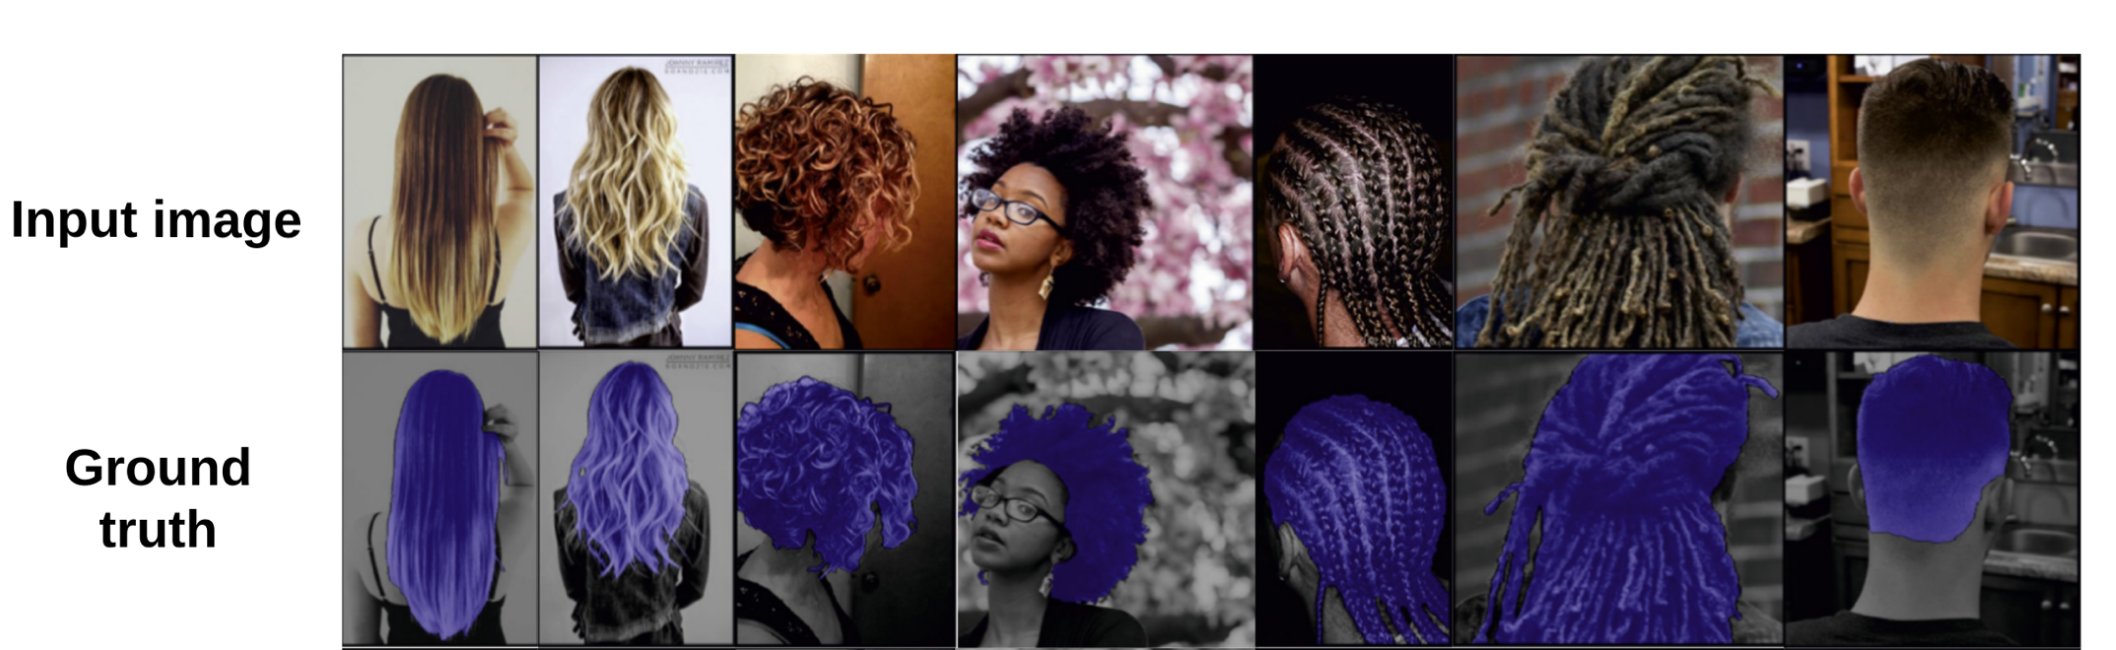
\includegraphics[width=0.9\textwidth]{chapter1/image/hair seg.png}
    \caption{Illustration for hair segmentation task. Hair masks is blue in color.}
    \label{fig:c1hairseg}
\end{figure}

With deep learning applied, this problem has been on the way to get an advanced performance in understanding image data. In addition to accuracy, the extent of media has also been extended to cover not just 2D images but also 3D images, videos, and so on. Apart from that, the field of deep learning possesses active communities and professional support. Tools for developing deep learning applications, such as Tensorflow, PyTorch, Caffe, were built in a modular way with a thorough document that makes development and engineering much more efficient. 
\par

Prior to the deep learning revolution, traditional image processing algorithms were used for both hair and clothes segmentation, but with deep learning, features are obtained automatically. Recent DNNs for hair segmentation are FPN \cite{fpn}, DenseNet \cite{densenet}, DeepLabv3 \cite{deeplabv3}. Aside from architecture, a hair matting technique utilizing image gradient is introduced in \cite{hairseg2matting}, playing the role of an auxiliary loss. Researchers also make an effort to apply filters to treat coarse masks \cite{hairseg2matting}. About clothing segmentation problem, Mask R-CNN \cite{maskrcnn}, Match R-CNN \cite{deepfashion2} are proposed to achieve instance segmentation in spite of complex architecture. The thesis work will exploit the start-of-the-art solution for hair and cloth segmentation tasks to achieve the thesis's goals. 
\par
\paragraph{Problem of real-time segmentation on mobile devices}

DNNs for segmentation are complex and require high memory usage and computational resources. Therefore, the main platforms to run these models must have a powerful computational unit (e.g., GPU support) or cloud. For instance, mobile applications often send input and receive output from Firebase, where developers push their DNNs. However, researchers recently realize the benefits of bringing deep learning toward the edge that includes devices with less power and resources. It ranges from user experience, offering anytime, anywhere access, with the great advantages of security, privacy, and energy consumption. \par

Discovering advantages from running DNNs on edge, big technology companies have been developing more and more frameworks to deploy models locally. A few must-mentioned frameworks for deep learning on mobile phones are TFLite, OONX, CoreML, PyTorch Mobile. Almost all frameworks for smartphones concern about optimization level, binary size, and supported hardware. Take the QNNPACK library \cite{qnnpack} for example, it is a mobile-optimized library for low-precision high-performance neural network inference. QNNPACK also provides the implementation of common neural network operators on quantized 8-bit tensors. Moreover, models developed especially for mobile also raise in the number; some of them are introduced in \textbf{section \ref{sec:cnn}}. 




\section{Objective and Contributions}

The thesis focuses on creating an Android app for the beauty field, aiming at smoothness and efficiency. By providing a real-time interaction experience, users see immediate feedback on objects they are tracking (at here are hair and clothes). In detail, users can preview images taken from cameras with hair or clothes being recolored and select a color as they like. Afterward, users are able to save or share images with hair and clothes recolored into storage. As a part of this thesis study, it is to research two crucial components: a fast on-device running model and a well-designed mobile app. Later, the problem in combining these two components is also seriously raised and tackled in my thesis. All in all, real-time performance on a wide variety of mobile devices is prioritized, while pixel-perfect masks may not be provided. \par
There are two main contributions of the thesis: a real-time beauty camera app running on Android and two deep learning models adapted for smartphones. About the app, it is designed with ten basic use cases, two of them are main features, namely Clothes Camera and Hair Camera. The real-time camera based on the CameraX framework achieves the speed of 60 FPS. In terms of masks rendering, I propose two methods (Bitmap and OpenGL), bringing about a good enough user experience. For rendering hair and clothes masks, it takes 24ms with OpenGL and slower with Bitmap. About the hair and clothes segmentation models, these two models achieve  86\% IoU on average. \par
\section{Difficulties} 
Hair can be classified into many categories, light or dark, curl or straight, etc. Therefore, many hair segmentation models can recognize hair in black or yellow but fail to the other colors. In addition to multiple variants, hair has an unstable and complex structure, unlike many objects with simple shapes. In terms of clothing, the color and shape of it are also incredibly various. Covering all these possibilities will lead to hardship in hair and clothing recognition, which ought to be resolved in the thesis work.


Nevertheless, smartphones usually constrain the memory of 4 gigabytes in total; thus, standard models would consume a large proportion of memory space. Also, long inference time of standard models is problematic, although hardware accelerators come into handy. One other difficulty in running models on mobile devices is that the size of the output mask is different from the size of the screen. Because of this mismatch, we have to rescale and meticulously render predictions to fit the screen. Furthermore, it is also essential to ensure that pipelines runs consistently on targeted environments and produces identical results with the inputs stay the same. 



\section{Thesis structure}

There are totally five chapters in this thesis proceeded as follows. \par 
\textbf{Chapter 1: Introduction.} This chapter gives an overview of the thesis work, presents reasons and motivations of the work. Besides, some lately advancements in the field of semantic learning, smartphone deployment is briefly introduced. After this chapter, readers get a view of difficulties in hair and clothes segmentation, aside from objectives that the thesis follows.  \par
\textbf{Chapter 2: Background.} This chapter firstly introduces some convolutional neural networks that have been deployed on mobile devices, along with their specific applications. Secondly, Android and a few libraries are presented; it is also mentioned the reasons why they are used. Finally, tools for model deployment are given basic understand with TFLite is the core. TFLite is described with model optimization and converter.  \par
\textbf{Chapter 3: Method.} 
This chapter explains the architecture of the proposed model, the app pipeline. For the DNN, it is also explained the reasons why the architecture is chosen. For the app, we provide a brief introduction of hardware accelerator and TFLite backend support. At last, two rendering methods are presented. \par
\textbf{Chapter 4: Experiments and Result.} This chapter indicates experiments conducted on both the app and the model, gives quantitative results after that. Finally, this chapter concludes the thesis and suggests future work.\par
\setcounter{page}{1}
% target: 6 pages
\mychapter{1}{CHAPTER 1. INTRODUCTION}\label{ch:chap1}
\graphicspath{{./chapter1/image/}}

Recommendation systems have been applied in a vast range of industries, ranging from retail to healthcare, and it is undoubtedly getting more and more popularized in the next few decades. Many recommender systems leveraged by artificial intelligence has reinforced users’ selection and brings about superhuman solutions. In such a background, a hair and clothes color recommendation system that helps them select the most suitable color is in desire of society.  Hair and cloth segmentation models are addressed as the core of this thesis; they, in this study, are proposed and assessed. From that, the thesis proposes a prototype for beauty apps, including use-case analysis, interface and architecture design. Afterward, real-time hair and cloth recoloring application for mobile devices is developed and finally evaluated. \par

\section{Motivation}
It is true that the clothing industry is in the top-4 most lucrative fields and often accounts for a significant portion of personal expenditures. People nowadays want to look good and expect higher at their outfits as the standard of living rises across the world. As a result, many find their preferred models, cuts, and styles of clothing but do not know what colors are the most well-suit to buy. These colors must flatter your skin tone or match with accessories’ tones. For a good outfit, pieces of clothes should not have any pair of complementary colors such as blue vs. orange, red vs. green. Usually, these color theories are well understood by stylists and fashionistas.
\par
Nevertheless, in case they choose a wrong color, many consequences might arise from that. Clothing that is not preferable is less likely to be worn, or more seriously, be discarded. Furthermore, it would form consumerism among society when people have not figured out suitable outfits, consequently increasing our environmental footprint. According to a report, the apparel industry's environmental impact, which is calculated throughout the entire life cycle of clothing, occupied 20\% of global water waste and 10\% of global carbon emission \cite{carbonemission}. Selecting clothes color visually on mobile phones is incredibly beneficial to the fashion industry.\par

Both women and men wear their hair in a variety of styles; each haircut can be dyed to many colors. With a multitude of colors, people always are often confused about commit a color from the wide variety available to them. 
\par
Considering the reasons mentioned earlier, there exists a need for a beauty app that helps the client to save time and effort in choosing hair and clothes color. Additionally, hair segmentation information can not only advance recommendation systems, but it is also used for a variety of applications, such as photo editing, make-up changes, and face detection. Further uses of clothing segmentation information appear on virtual try-on, clothing retrieves system, all of which are valuable applications for everyone in daily life.
\par
\section{Problem background} \label{sec:pb}

Augmented reality is an emerging technology, and it provides users with an interactive experience in both the physical and digital worlds. An augmented reality system aims at creating a real-time modification of the real-world environment for an interactive experience. Augmented reality continues to proliferate and become pervasive among a wide range of applications, including beauty. In the beauty industry, where live virtual try-on of beauty products is of great importance, augmented reality involves overlaying visual information onto real scenes so that not only user’s experience enhances, but companies also promote their products. To advance this domain, the segmentation task plays a key role.
\par
Semantic image segmentation, the task of mapping each pixel to a label, is a major and old challenge in the area of computer vision. Image segmentation can be treated as pixel-level prediction because it classifies each pixel into its category. With hair, segmentation problem strives for even fine details of strands of hair and avoid confusion between skin and hair. In the clothes segmentation problem, the output is a semantic analysis showing which clothing items are present, where in the image these are, and what shape they have.

\begin{figure} [H]
    \centering
    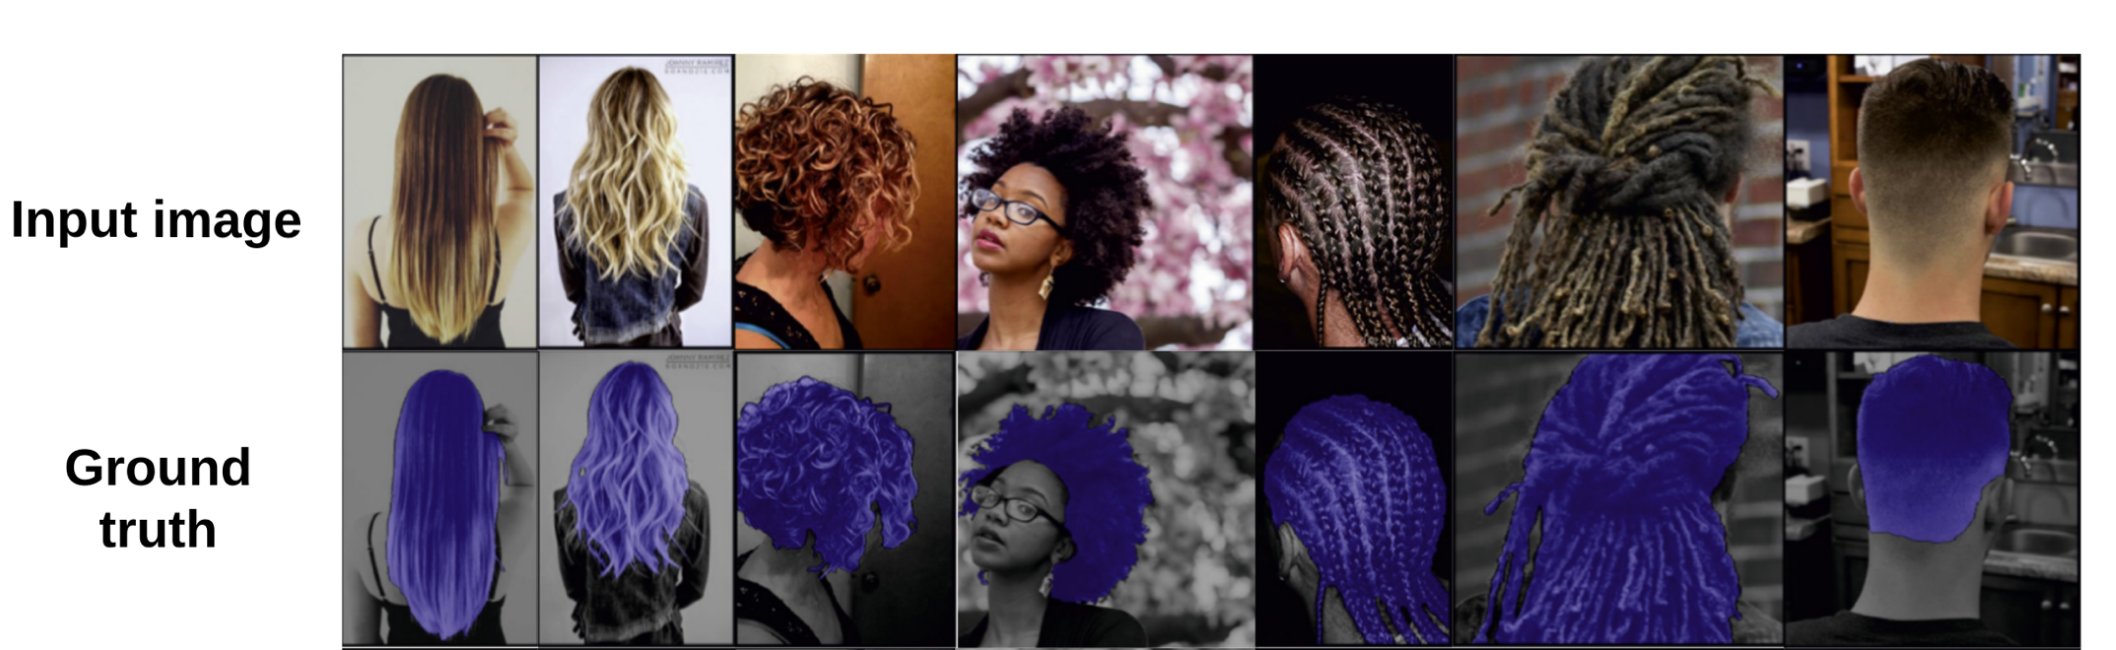
\includegraphics[width=0.9\textwidth]{chapter1/image/hair seg.png}
    \caption{Illustration for hair segmentation task. Hair masks is blue in color.}
    \label{fig:c1hairseg}
\end{figure}

With deep learning applied, this problem has been on the way to get an advanced performance in understanding image data. In addition to accuracy, the extent of media has also been extended to cover not just 2D images but also 3D images, videos, and so on. Apart from that, the field of deep learning possesses active communities and professional support. Tools for developing deep learning applications, such as Tensorflow, PyTorch, Caffe, were built in a modular way with a thorough document that makes development and engineering much more efficient. 
\par

Prior to the deep learning revolution, traditional image processing algorithms were used for both hair and clothes segmentation, but with deep learning, features are obtained automatically. Recent DNNs for hair segmentation are FPN \cite{fpn}, DenseNet \cite{densenet}, DeepLabv3 \cite{deeplabv3}. Aside from architecture, a hair matting technique utilizing image gradient is introduced in \cite{hairseg2matting}, playing the role of an auxiliary loss. Researchers also make an effort to apply filters to treat coarse masks \cite{hairseg2matting}. About clothing segmentation problem, Mask R-CNN \cite{maskrcnn}, Match R-CNN \cite{deepfashion2} are proposed to achieve instance segmentation in spite of complex architecture. The thesis work will exploit the start-of-the-art solution for hair and cloth segmentation tasks to achieve the thesis's goals. 
\par
\paragraph{Problem of real-time segmentation on mobile devices}

DNNs for segmentation are complex and require high memory usage and computational resources. Therefore, the main platforms to run these models must have a powerful computational unit (e.g., GPU support) or cloud. For instance, mobile applications often send input and receive output from Firebase, where developers push their DNNs. However, researchers recently realize the benefits of bringing deep learning toward the edge that includes devices with less power and resources. It ranges from user experience, offering anytime, anywhere access, with the great advantages of security, privacy, and energy consumption. \par

Discovering advantages from running DNNs on edge, big technology companies have been developing more and more frameworks to deploy models locally. A few must-mentioned frameworks for deep learning on mobile phones are TFLite, OONX, CoreML, PyTorch Mobile. Almost all frameworks for smartphones concern about optimization level, binary size, and supported hardware. Take the QNNPACK library \cite{qnnpack} for example, it is a mobile-optimized library for low-precision high-performance neural network inference. QNNPACK also provides the implementation of common neural network operators on quantized 8-bit tensors. Moreover, models developed especially for mobile also raise in the number; some of them are introduced in \textbf{section \ref{sec:cnn}}. 




\section{Objective and Contributions}

The thesis focuses on creating an Android app for the beauty field, aiming at smoothness and efficiency. By providing a real-time interaction experience, users see immediate feedback on objects they are tracking (at here are hair and clothes). In detail, users can preview images taken from cameras with hair or clothes being recolored and select a color as they like. Afterward, users are able to save or share images with hair and clothes recolored into storage. As a part of this thesis study, it is to research two crucial components: a fast on-device running model and a well-designed mobile app. Later, the problem in combining these two components is also seriously raised and tackled in my thesis. All in all, real-time performance on a wide variety of mobile devices is prioritized, while pixel-perfect masks may not be provided. \par
There are two main contributions of the thesis: a real-time beauty camera app running on Android and two deep learning models adapted for smartphones. About the app, it is designed with ten basic use cases, two of them are main features, namely Clothes Camera and Hair Camera. The real-time camera based on the CameraX framework achieves the speed of 60 FPS. In terms of masks rendering, I propose two methods (Bitmap and OpenGL), bringing about a good enough user experience. For rendering hair and clothes masks, it takes 24ms with OpenGL and slower with Bitmap. About the hair and clothes segmentation models, these two models achieve  86\% IoU on average. \par
\section{Difficulties} 
Hair can be classified into many categories, light or dark, curl or straight, etc. Therefore, many hair segmentation models can recognize hair in black or yellow but fail to the other colors. In addition to multiple variants, hair has an unstable and complex structure, unlike many objects with simple shapes. In terms of clothing, the color and shape of it are also incredibly various. Covering all these possibilities will lead to hardship in hair and clothing recognition, which ought to be resolved in the thesis work.


Nevertheless, smartphones usually constrain the memory of 4 gigabytes in total; thus, standard models would consume a large proportion of memory space. Also, long inference time of standard models is problematic, although hardware accelerators come into handy. One other difficulty in running models on mobile devices is that the size of the output mask is different from the size of the screen. Because of this mismatch, we have to rescale and meticulously render predictions to fit the screen. Furthermore, it is also essential to ensure that pipelines runs consistently on targeted environments and produces identical results with the inputs stay the same. 



\section{Thesis structure}

There are totally five chapters in this thesis proceeded as follows. \par 
\textbf{Chapter 1: Introduction.} This chapter gives an overview of the thesis work, presents reasons and motivations of the work. Besides, some lately advancements in the field of semantic learning, smartphone deployment is briefly introduced. After this chapter, readers get a view of difficulties in hair and clothes segmentation, aside from objectives that the thesis follows.  \par
\textbf{Chapter 2: Background.} This chapter firstly introduces some convolutional neural networks that have been deployed on mobile devices, along with their specific applications. Secondly, Android and a few libraries are presented; it is also mentioned the reasons why they are used. Finally, tools for model deployment are given basic understand with TFLite is the core. TFLite is described with model optimization and converter.  \par
\textbf{Chapter 3: Method.} 
This chapter explains the architecture of the proposed model, the app pipeline. For the DNN, it is also explained the reasons why the architecture is chosen. For the app, we provide a brief introduction of hardware accelerator and TFLite backend support. At last, two rendering methods are presented. \par
\textbf{Chapter 4: Experiments and Result.} This chapter indicates experiments conducted on both the app and the model, gives quantitative results after that. Finally, this chapter concludes the thesis and suggests future work.\par
\setcounter{figure}{0}
\mychapter{2}{CHAPTER 2. BACKGROUND}\label{ch:chap2} 


\section{Convolutional Neural Networks applications} \label{sec:cnn}

Convolutional neural network (CNN or ConvNet) is a class of deep neural networks often applied to analyzing visual imagery. CNN is based on multi-layer neural networks that learn relevant features from images using filters, performing several tasks like object classification, detection, and segmentation. Concretely, early versions of CNN are good at classifying handwritten digits, fruits, animals, etc. Commonly, CNN is made up of three types of layer: Convolution layer, Pooling layer, and Fully-connected layer. 

\begin{figure} [H]
    \centering
    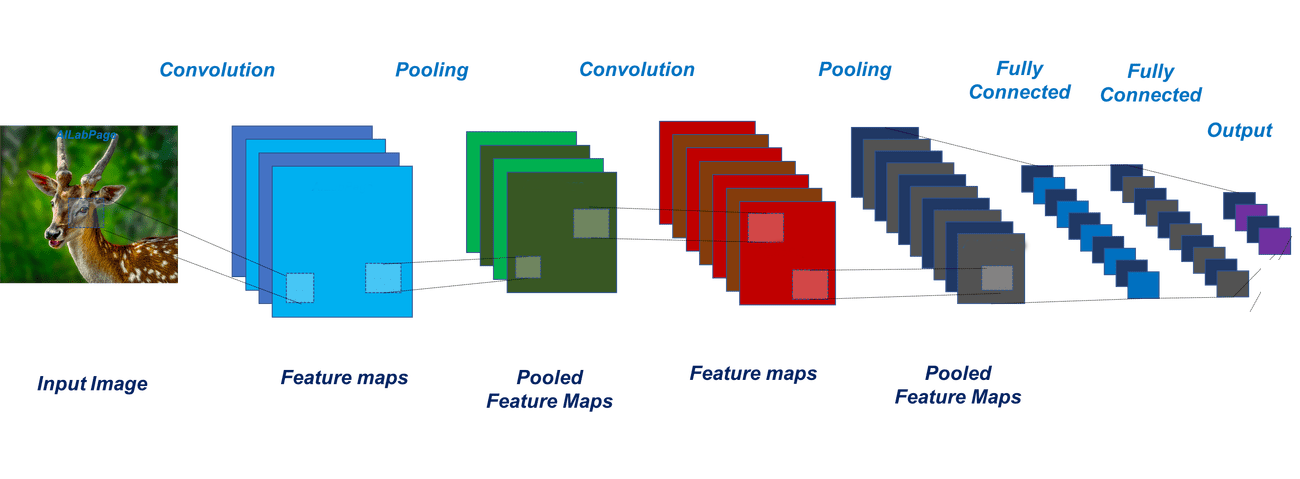
\includegraphics[width=0.9\textwidth]{chapter2/image/CNN.png}
    \caption{General architecture of CNN}
    \label{fig:cnn}
\end{figure}

Some popular architectures in the field of CNN are VGG \cite{vgg}, ResNet \cite{resnet}. Although they have a high accuracy score in computer vision tasks, they fail to run on mobile devices as they have high latency. Next in this section, some models that are capable of running on mobile phones are presented. I divide them according to tasks: object classification, object detection, and object classification.

\subsection{Object classification}
Object classification involves taking an input image and outputting a class that the image falls under. \textbf{Figure \ref{fig:cnn}} is an example of a classification network, where animals are classified. Head of classification models usually consists of fully-connected layers. The number of classes is often equal to the number of neural at the last layer. \par

Some popular image classification models are ResNet, Inception, PyramidNet. However, they require heavy computational resources, are often run on GPU. Models deployed on mobile devices often have simpler architecture and smaller size. Some of them are MobiNetv2 \cite{mobilenetv2}, MobiDets \cite{mobiledets}. These models have been used for some applications on smartphones like flower classification, food classification.


\subsection{Object detection}
Object detection aims at identifying objects of interest in images. Existing models can be categorized into two-stage detectors and one-stage single shot
detectors. For two-stage detectors, including R-FCN, ThunderNet \cite{thundernet}, region proposals must be generated first before the detector can make any subsequent predictions. Two-stage detectors are not efficient in the inference phase due to this multi-stage nature. 

On the other hand, one-stage single shot detectors, such as SqueezeDet \cite{squeezenet}, SSD, YOLO, require only one single pass through the network to predict all the bounding boxes, making them ideal candidates for efficient inference on edge devices. Among them, SSDLite is an efficient variant of SSD that has become one of the most popular lightweight detectors on the smartphone. 

\begin{figure} [H]
    \centering
    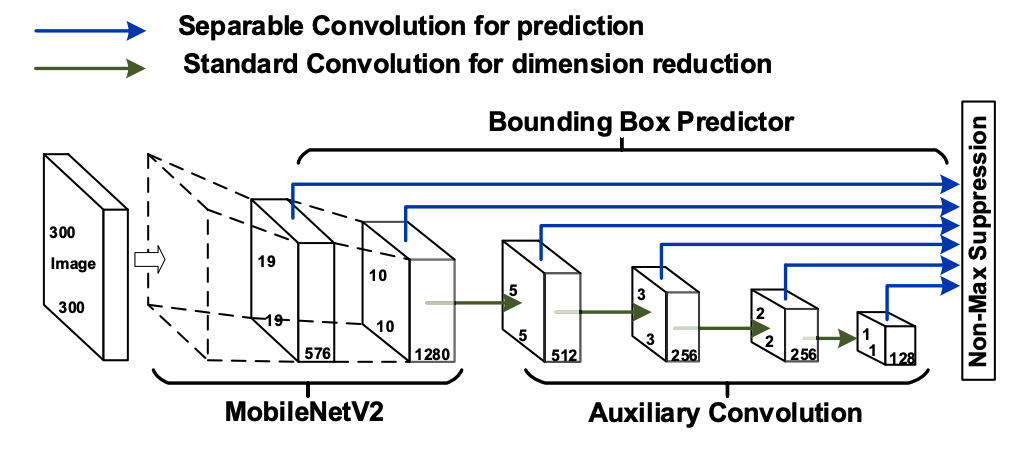
\includegraphics[width=0.9\textwidth]{chapter2/image/ssdlite.png}
    \caption{The network architecture of MobilNetV2-SSDLite}
    \label{fig:cnn}
\end{figure}

SSDLite is a general-purpose model; some applications of it are license plate detection, car detection, face detection, hand detection, to name but a few.

\subsection{Object segmentation}
ConvNets are widely used for segmentation problem, which is already introduced in \textbf{section \ref{sec:pb}}. Most modern models for segmentation are composed of two components: upsampling and downsampling. \par
\begin{figure} [H]
    \centering
    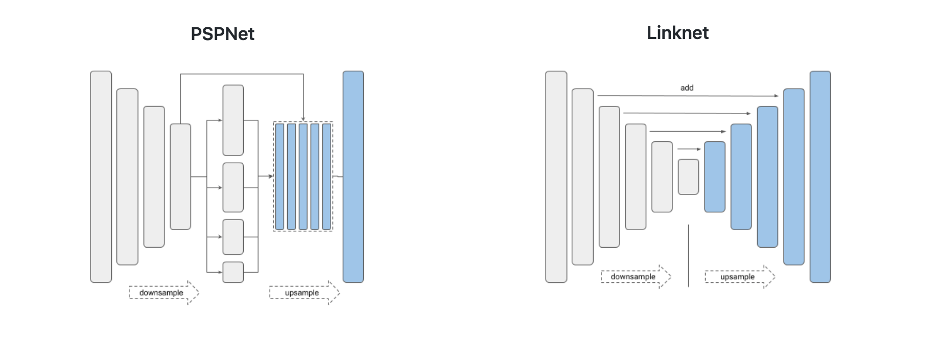
\includegraphics[width=0.9\textwidth]{chapter2/image/segnet.png}
    \caption{Architecture of modern segmentation models}
    \label{fig:my_label}
\end{figure}
While upsampling encodes the input image into feature representations at multiple levels, downsampling is to restore the condensed feature map to the original size of the input image. There are many semantic segmentation networks that have high accuracy such as Mask R-CNN \cite{maskrcnn}, SegNet\cite{segnet}, PSPNet\cite{pspnet}, but poor about speed. For instance, PSPNet which uses pyramid pooling module for more reliable prediction has 65.7 million parameters and runs at about 1 FPS.  \par

Recent approach for the task of object segmentation is \textbf{DeepLabv3+} - an extension of DeepLabv3 in encoder-decoder structure. In general, DeepLabv3 is used as an encoder. The encoder module encodes multi-scale contextual information by applying atrous convolution at multiple scales. This architecture is able to perform several parallel atrus convolution with different rates. Meanwhile, the decoder module refines the segmentation results along object boundaries. \par

\begin{figure} [H]
    \centering
    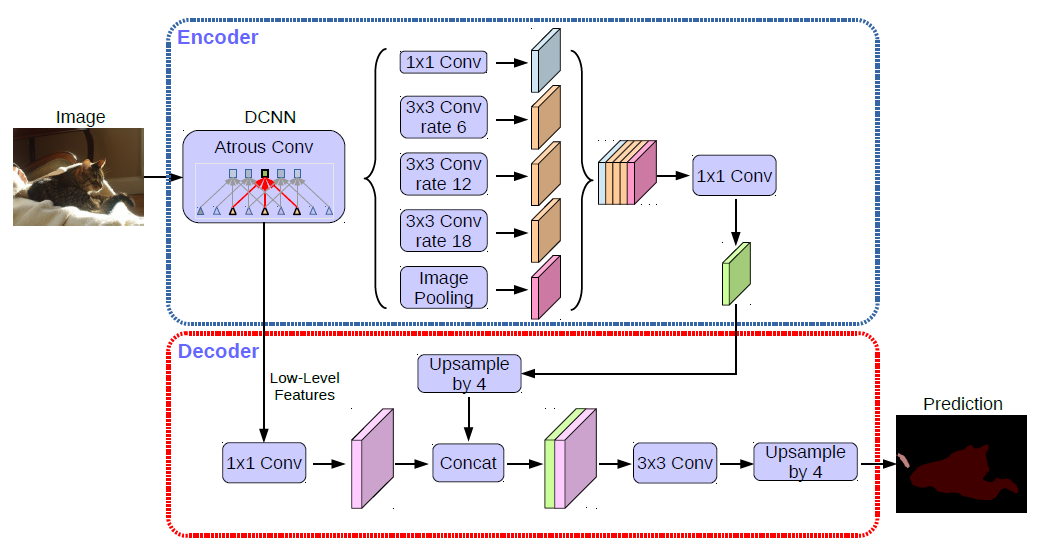
\includegraphics[width=0.8\textwidth]{chapter2/image/deeplab.png}
    \caption{DeepLabv3+ architecture for segmentic segmentation. Source \cite{deeplabv3plus}}
    \label{fig:my_label}
\end{figure}

In fact, applications of segmentation models on smartphones are manifold, ranging from road scene segmentation to human segmentation to style transfer. In the next chapter, I will propose a lightweight segmentation model that aims to recognize hair and clothes. \par




\section{Android} \label{sec:android}

Android is the most popular operating system for smartphones and tablets, developed by Google. According a market share report in 2019, there is 74.2\% of cellphones across the world running Android, including top smartphone vendors like Samsung, Sony, Oppo... \par

Released in 2008, since then, Android is still open-source under Apache licenses. This openness is one of the most appreciated aspects of Android. As the source code is revealed to the public, many developers around the world are able to not only have a better understanding of what is happening in the background but also to actively contribute to the project. Until now, this platform has over ten versions with many different enhancements after each. Starting with the smartphone, now Android also are presented on smart Tv, Smart Watch, Car, and many other embedded devices. \par

\begin{figure} [H]
    \centering
    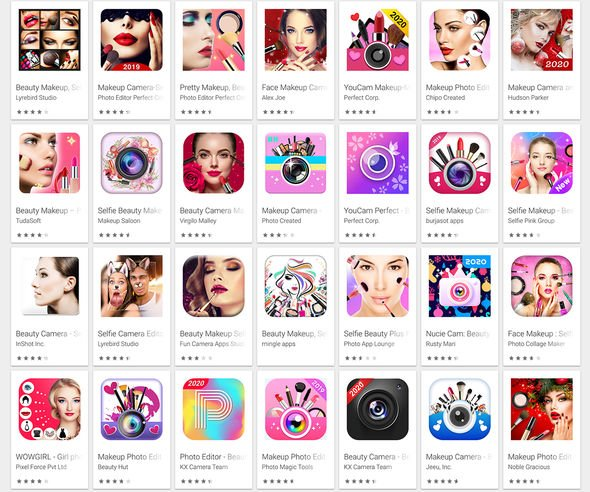
\includegraphics[trim=20 40 20 40,clip,width=0.9\textwidth]{chapter2/image/chplay.jpeg}
    \caption{Search results for "Beauty apps" on Google Play Store}
    \label{fig:android}
\end{figure}


\noindent Some features that make Android become much more popular than other smartphone operating system is:
\begin{itemize}
    \item 
	Android is highly customizable because it is an open-source operating system. It can be edited on its own without interference from Google. Can run on many devices with different processing architectures
\item	Java program language, which is chosen as main development, is easy to learn and write. Moreover, Java is a class-based and highly object-oriented program language so that it is able to accommodate big projects. Especially, Java has many powerful libraries; hence Android can take advantages from them.
\item	The developer community is large and supportive.
\end{itemize}

An Android app is shipped as an Android Package (APK) that contains different files. It contains the Android manifest specifying the app’s starting point, the executable code, the developer key, and the resources needed to run the app. If the app consists of any machine learning model, such models will be attached as a resource. After the app is packaged under the \emph{“.apk”} extension, an APK file can be public for users to download by using Google Play Store (has over 3 million apps are available there). \par

\subsection{AndroidX} \label{sec:androidx}

AndroidX is a major improvement to the original Android Support Library, which is no longer maintained. In other words, AndroidX provides new tools and libraries under the \verb|androix.*| namespace, while old packages taken from the Android Support Library are mapped to this new namespace. 
More supportive, all Jetpack components are packaged into AndroidX. Jetpack is a suite of libraries to help developers follow best practices, and make great Android apps that works consistently across Android versions and devices so that developers can focus on the code they care about. \par

\subsection{CameraX} \label{sec:camerax}

It is vital to handle cameras to get media data for the latter phases, capture the photos from the front or rear camera. Therefore, choosing an external library seems reasonable because it would be more reliable in case deploying in heterogeneous landscapes and device hardware. After investigating several camera libraries, such as camera2, PreviewCam, I choose CameraX as the app can make use of the Preview and Analysis user cases; thus, the app would reduce a substantial amount of code.\par

CameraX was first introduced in Google I/O 2019 as a Jetpack library, to meet the increased requirement of functionality for the camera. Meanwhile, the complexity and effort of the implementation would also be reduced considerably. CameraX inherits from Camera2 API, but with ease of use. It uses a simpler approach that is lifecycle-aware and is based on use cases. \par

CameraX's use cases allow you to focus on the task you need to accomplish instead of spending time covering device-specific settings. Three essential use cases of CameraX are: \par
\begin{itemize}
\item	Preview use case can be used to provide a preview of the current camera stream within a \emph{SurfaceTextureView}. This view is then connected to a corresponding \emph{TextureView} to display the camera content on screen. 
\item  Image analysis use case provides a CPU-accessible image to carry out image processing or machine learning inference. The image will be executed through the \emph{analyze()} method which runs on each frame.
\item	Image capture use case is used for low latency image captures. There are a number of options that we can set for the camera in this use case.
\end{itemize}



% thieu: Tensorlfow-Converter

\section{Model deployment}
The thesis introduced a few CNNs developed for mobile devices; the Android platform and accompanied libraries were also indicated. The thesis will give an overall view of ML models deployment on both servers and mobile phones in the section below. 

\subsection{Deployment on Server/Cloud Platforms}
Some frameworks (e.g., Tensorflow Serving, Triton) and platforms (e.g., Google Cloud ML Engine, Amazon SageMaker) can facilitate this deployment. The following figure illustrates how to serve deep learning models on cloud/server.

\begin{figure} [H]
    \centering
    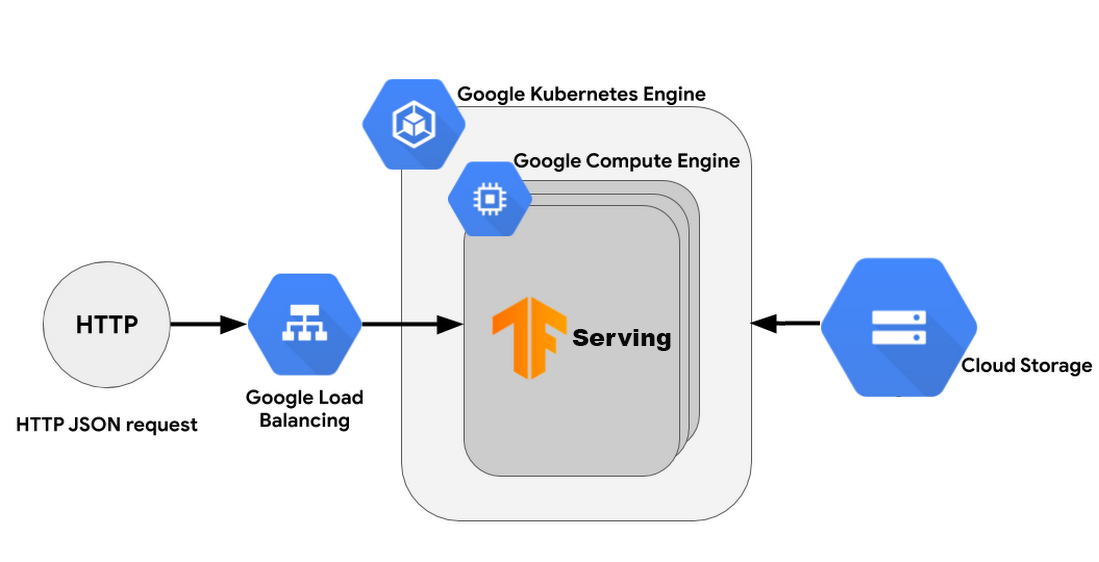
\includegraphics[width=0.9\textwidth]{chapter2/image/tfserving.png}
    \caption{Model deployment on Google Cloud}
    \label{fig:cloud}
\end{figure}

\paragraph{TF Serving}
TF Serving \cite{tfserving} is a deep learning framework specially designed to deploy deep learning models to servers. It operates as a set of processes on one or more network servers, using one of several advanced architectures to handle synchronization and distributed computation. To communicate with TF Model Server, clients are allowed to send inputs and receive outputs through REST or gRPC interfaces. \par 
\paragraph{Google Cloud ML Engine}
Google Cloud ML Engine \cite{googlecloudml} is a popular cloud platform for deploying deep learning software and training deep learning models. To deploy a trained model, the first step is to upload your saved model to a Cloud Storage bucket. After that, TF Serving , installed on all virtual machines in that cluster, loads the model to memory, executes it, and responds to clients. Other more convenient ways to deploy ML models provided by Google are Cloud Functions \cite{cloudfunctions}, and AI Platform Predictions \cite{platformprediction}.
These solutions assist the deployment of your models at scale to get predictions from the cloud, which hosts your model for online and batch prediction requests. \par
%warm invoke


\subsection{Deployment on Mobile Platforms}
In this section, the thesis talks about the deployment of ML models on smartphones through introducing the TFLite framework. Firstly, we start with some basic information about this framework. After that, we get a brief view of optimization and adaptation techniques that this framework provides to convert models for on-device inference. \par
\subsubsection{Tensorflow and TFLite}
Tensorflow is the name of a well-known deep learning framework. It is debuted at Google I/O Conference in 2016 as an opensource. After that, it has received goods feedbacks from developer community for its computational supportability and flexible uses for both research and industry. \par

Following the success, Tflite was adapted as a software stack specifically for mobile development in May 2017. Until now, it becomes prevalent and supports both two main mobile OS: iOS and Android. With this comprehensive framework, developing and training new networks for machine learning tasks has become increasingly more reasonable. \par

Both Tensorflow and TFlite are open-source and cross-platform; hence developers are free to clone the source code from Github and build it manually with Bazel afterward. For that, any modifications to operators, targeted architecture, etc., are permissible. This is two commands used to build TFLite: \par

\begin{verbatim}
bazel build -s -c opt --strip always --cxxopt='--std=c++11'
--config=android_arm64 //tensorflow/lite:libtensorflowlite.so

bazel build -s -c opt --strip always --cxxopt='--std=c++11' 
--config android_arm64 //tensorflow/lite/delegates/gpu:
libtensorflowlite_gpu_delegate.so    
\end{verbatim}


All of the above commands are used to build the TFLite library for $arm64-v8a$. The difference is that the first one is to build a shared library for the CPU backend, while the second one is for the GPU backend. In fact, Tflite supports almost major architecture, such as: $armabi$, $armabi-v7a$, $x86$, $x86\_64$. One other benefit of TFLite is that it is compatible with multiple hardware, such as EdgeTPU, NNAPI,  GPU, CPU. \par

\subsubsection{TFLite Converter}\label{subsec:converter}

TFLite Converter is a built-in module, already included in the TFlite framework, executing conversion to light-weight models for edge devices. The converter inputs TensorFlow models and outputs an efficient form for use by the interpreter. In more detail, the converter optimizes the model and then converts to a FlatBuffer, an efficient storage format which can be read later using the TFLite Interpreter on mobile devices. \par

\begin{figure}[H]
    \centering
    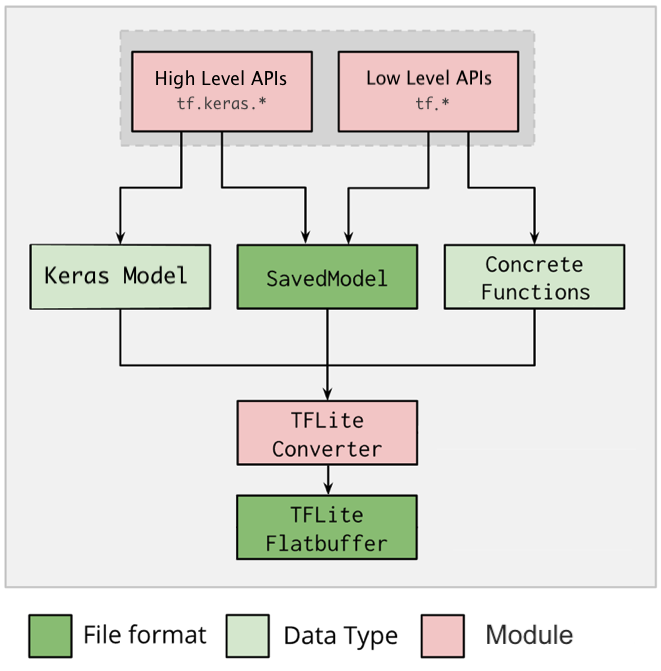
\includegraphics[width=0.6\textwidth]{chapter2/image/tflite3.png}
    \caption{Workflow of TFLite Converter}
    \label{fig:tflite}
\end{figure}
 
The above figure shows steps to convert a Tensorflow model to a TFLite model. As you can see, TFLite Converter only supports several specific saved model formats, which will be listed later. In addition, unsupported and un-predefined operations also cause critical errors, so these must be written in C++ code using Tensorflow C++ API or discarded from the model, so in order to use converter, we need to meet all requirement of input format and architecture.\par 

In relevant to input format requirements, TFLite Converter only supports conversion for three types of data: Keras Model (*.h5), SavedModel (a directory), and Concrete Functions (source code). If you use the version 1, you have additional options: GraphDef from a session or Frozen GraphDef from a file) However, it is deprecated in the version 2 and would not be introduced here. Furthermore, TFlite has restrictions in data type; data of unsupported data type must be cast to a supported one. The prescribed data types are Float32, Int32, Int64, and unsigned Int8. \par


\subsubsection{Quantization} \label{subsec:quantization}
Quantization is one of a few model optimization techniques that is usually used during the conversion of a Tensorflow to a TFLite model. Technically, quantization is the process of assigning values from a large set to values in a smaller set, used here as a technic to change data types. Take conversion from \emph{float32} to \emph{float16} for an example, quantization here is referred to as reducing the precision of a model’s weights; consequently, the memory required to store a parameter is 2 bytes instead of 4 bytes. Hardware support for \emph{int8} computations is typically 2 to 4 times faster when compared to for \emph{float32} computations. Additionally, as there are less data to transport, processors can execute operations with less precise numbers much faster. \par

Quantization can be integrated into training (called quantization aware training) or the post-training phase. More various, models are flexible to only be quantized on weights only or both weights and activations. The following is the equation of a general one: \par

\begin{equation}
    output = (input - min\_range) * \frac{range(data\_type)}{(max\_range - min\_range)}
\end{equation}
Where \begin{itemize}
    \item [$-$] $input$: Value is about to be quantized
    \item [$-$] $min\_range$: Minimum value in the range of input
    \item [$-$] $max\_range$: Maximum value in the range of input
    \item [$-$] $range(data\_type)$: Equals to $max(data\_type) - min(data\_type)$
    \item [$-$] $output$: Value after being quantized
\end{itemize} 

Assume the data type is \emph{float} and has a possible range of [0.0, 10.0] and the quantized data type has an \emph{uint8} range of [0, 255]. In this case, quantizing from \emph{float} to \emph{uint8} will multiply each value by 255/8 and cast to \emph{uint8}. \par

Although quantization is efficient to make the neural networks faster and smaller, this optimization can potentially result in a slight reduction in accuracy, which must be considered during development process. Besides quantization, TFLite Converter provides other powerful optimization techniques, taking weigh pruning and weight clustering for example. They are not introduced in this thesis, though. \par



\setcounter{figure}{0}
% thiếu: 3.3, 3.2
% target: 15 pages
\mychapter{3}{CHAPTER 3. METHODS} \label{ch:chap3} \graphicspath{{./chapter3/image/}}

This chapter proposes a general pipeline for on-device vision applications and a method based on deep learning solving hair segmentation and clothing segmentation tasks. Aside from that, methods for overlaying a mask on a photograph are also demonstrated. \par
Concerning the pipeline for the Android application, I first list all use cases for the app and then do further analysis on them. With some intricate use cases having many classes involved, sequence diagrams are provided to illustrate how these classes work together. Such generic prototypes can be reused later, whenever camera application development is needed. \par
In terms of the deep learning model, every component of the proposed network will be explained in this chapter. The proposed method for optimizing the model and converting it to TFLite's supported format will also be presented. The practical performance and accuracy of the proposed method will be discussed in the next chapter.\par

\section{Use-Case Analysis and Design} \label{sec:usecase}

\subsection{Use Case}
This sector defines the functional requirements for the app. In summary, the app has \textbf{1 actor} and \textbf{10 use cases}. An actor models a type of role played by an entity that interacts with the app. The actor can be a human user or an external system. Meanwhile, a use case describes a sequence of interactions between actors and systems to accomplish a particular goal. Use cases are usually referred to as system functionalities that a system should perform in interaction with one or more external users (actors). In the case of the thesis, the actor is the users, and the system is the mobile application. The figure below is the proposed UML \cite{uml} use case diagram: \par

\begin{figure} [H]
    \centering
    \captionsetup{justification=centering}
    \includegraphics[width=1.0\textwidth]{chapter3/image/use-case.png}
    \caption{Use case diagram for the hair and clothes app}
    \label{fig:schnet_LiNet}
\end{figure}

With each use case, it is accompanied by a table describing it. In tables, the "Pre-condition" row is a list of conditions that must be met before the action of that use case. The "Post-condition" row is a list of conditions that must be reached after the action of that use case. The "Expected result" row lists acceptable results of that use case.

\begin{center} 
\begin{table} [H]
\caption{Hair camera use-case description} 
\begin{tabular}{p{0.35\linewidth} | p{0.6\linewidth}}
\hline
USER CASE            & UC-1 \\ \hline
Use case name        & Hair Camera   \\ \hline
Use case description & Real-time camera preview with hair \\ \hline
Pre-condition         &   User were in the app's main screen, selected the “Hair Camera” option. Request permissions must be accepted before camera starts \\ \hline
Post-condition        &   Camera preview is displayed in response to the hardware. Hair mask is overlayed directly on frames  \\ \hline
Basic flow           &   \begin{enumerate}
    \item User switches front to rear camera, and vice versa.
    \item User changes color of hair.
    \item User clicks the capture button.
\end{enumerate}   \\ \hline
Alternate flows      &   \begin{enumerate}
    \setcounter{enumi}{3}
    \item User clicks the back button
\end{enumerate}   \\ \hline
Expected result      &  \begin{enumerate}
    \item If permissions are not granted, ask for the permissions.
\end{enumerate}    \\ \hline
\end{tabular}
\end{table}
\end{center}


\begin{center}
\begin{table} [H]
\caption{Clothes camera use-case description} 
\begin{tabular}{p{0.35\linewidth} | p{0.6\linewidth}}
\hline
USER CASE            & UC-2 \\ \hline
Use case name        & Clothes Camera  \\ \hline
Use case description & Real-time camera preview with clothes recolored     \\ \hline
Pre-condition         &   User were in the app's main screen, selected the “Clothes Camera” option. Request permissions must be accepted before camera starts   \\ \hline
Post-condition        &   Camera preview is displayed in response to the hardware. Clothes mask is directly overlaied on frames   \\ \hline
Basic flow           &  \begin{enumerate}
  \item Users switch front to rear camera, and vice versa.
  \item Users change color for clothes.
  \item	Users click the capture button. 
\end{enumerate} \\ \hline
Alternate flows      &   \begin{enumerate}
    \setcounter{enumi}{3}
    \item User clicks the back button, returning to the main screen
\end{enumerate}   \\ \hline
Expected result      &  \begin{enumerate}
    \item If permissions are not granted, ask for the permissions
\end{enumerate}    \\ \hline
\end{tabular}
\end{table}
\end{center}


\begin{center}
\begin{table} [H]
\caption{Change lens use-case description} 
\begin{tabular}{p{0.35\linewidth} | p{0.6\linewidth}}
\hline
USER CASE            & UC-3 \\ \hline
Use case name        &  Change lens  \\ \hline
Use case description &   One button is responsible for switching between front and rear lens  \\ \hline
Pre-condition         &   Camera preview is displayed, but user want to the other camera instead   \\ \hline
Post-condition        &   Preferable camera lens is chosen. User is now ready for capture.   \\ \hline
Basic flow           &  \begin{enumerate}
  \item User clicks on lens switching button.
  \item	Preview camera displays image for the front camera if the rear camera is opening. 
  \item New mask is generated and replaces the old one.
\end{enumerate}    \\ \hline
Alternate flows      &   N/A   \\ \hline
Expected result      & \begin{enumerate}
    \item User is able to change between camera lenses multiple times.
\end{enumerate}     \\ \hline
\end{tabular}
\end{table}
\end{center}


\begin{center}
\begin{table} [H]
\caption{Capture use-case description} 
\begin{tabular}{p{0.35\linewidth} | p{0.6\linewidth}}
\hline
USER CASE            & UC-4 \\ \hline
Use case name        &  Capture \\ \hline
Use case description &  One button is responsible for capture from camera     \\\hline
Pre-condition         &   Camera preview is displayed, user switched to lens his/her want. Now, user want to capture the frame at that moment  \\ \hline
Post-condition        &   Frame is captured and ready for latter use  \\ \hline
Basic flow           &   \begin{enumerate}
    \item 	User clicks on capture button
\item Stop camera previewing
\item The frame at the moment is saved to memory
\item Show options to treat the captured frame
\end{enumerate}
\\ \hline
Alternate flows      & N/A     \\ \hline
Expected result      &  
\begin{enumerate}
    \item User is able to capture multiple times.
\end{enumerate}   \\ \hline
\end{tabular}
\end{table}
\end{center}


\begin{center}
\begin{table} [H]
\caption{Clothes segmentation use-case description} 
\begin{tabular}{p{0.35\linewidth} | p{0.6\linewidth}}
\hline
USER CASE            & UC-5 \\ \hline
Use case name        &  Clothes segmentation  \\ \hline
Use case description &  Clothes color in a chosen image is recolored    \\\hline
Pre-condition         &   User was in the app’s main screen, selected the “Clothes segmentation” option. Permission requests must be accepted before camera starts   \\ \hline
Post-condition        &   Input image is recolored and applied filter. User gets recolored image his/her want.   \\ \hline
Basic flow           &   \begin{enumerate}
    \item Choose an image from gallary
\item Choose color for clothes in image
\item Choose filter that is going to apply to the image
\item Save \& Share the new image
\end{enumerate}
   \\ \hline
Alternate flows      &    \begin{enumerate}
    \setcounter{enumi}{4}
    \item User clicks on Back button, return to the main screen
\end{enumerate}  \\ \hline
Expected result      &  \begin{enumerate}
    \item If user chooses unsupported file format, showing up this error
\item New image is saved and shared successfully
\end{enumerate}    \\ \hline
\end{tabular}
\end{table}
\end{center}

%finish

\begin{center}
\begin{table} [H]
\caption{Hair segmentation use-case description} 
\begin{tabular}{p{0.35\linewidth} | p{0.6\linewidth}}
\hline
USER CASE            & UC-6 \\ \hline
Use case name        &  Hair segmentation  \\ \hline
Use case description &  Hair color in a chosen image is recolored    \\\hline
Pre-condition         &   User was in the app’s main screen, selected the “Hair segmentation” option. Permission requests must be accepted before camera starts   \\ \hline
Post-condition        &   Input image is recolored and applied filter. User gets recolored image his/her want.   \\ \hline
Basic flow           &   \begin{enumerate}
    \item Choose an image from gallary
    \item Choose color for hair in image
    \item Choose filter that is going to apply to the image
    \item Save \& Share the new image
\end{enumerate}
   \\ \hline
Alternate flows      &    \begin{enumerate}
    \setcounter{enumi}{4}
    \item User clicks on Back button, return to the main screen
\end{enumerate}  \\ \hline
Expected result      &  \begin{enumerate}
    \item 	If user chooses unsupported file format, showing up this error
    \item 	New image is saved or shared successfully
\end{enumerate}    \\ \hline
\end{tabular}
\end{table}
\end{center}

\begin{center}
\begin{table} [H]
\caption{Hair color scanning use-case description} 
\begin{tabular}{p{0.35\linewidth} | p{0.6\linewidth}}
\hline
USER CASE            & UC-7 \\ \hline
Use case name        &  Hair color scanning  \\ \hline
Use case description &  Hair color on camera preview will continuously switch to all colors.    \\\hline
Pre-condition         &  User was in the app’s main screen, selected the “Hair color scanning” option. Permission requests must be accepted before camera starts    \\ \hline
Post-condition        &   User looked at his/her hair in different colors. User want to experience other user cases.   \\ \hline
Basic flow           &  \begin{enumerate}
    \item Camera opens, switching camera lens as user want
\item	Hair mask renders directly on camera preview

\end{enumerate}    \\ \hline
Alternate flows      &   \begin{enumerate}
    \setcounter{enumi}{2}
    \item User clicks on Back button, return to the main screen
\end{enumerate}   \\ \hline
Expected result      &  \begin{enumerate}
    \item Hair is recolored successfully
    \item User is able to change camera lens
\end{enumerate}    \\ \hline
\end{tabular}
\end{table}
\end{center}

\begin{center}
\begin{table} [H]
\caption{Select color use-case description} 
\begin{tabular}{p{0.35\linewidth} | p{0.6\linewidth}}
\hline
USER CASE            & UC-8 \\ \hline
Use case name        &  Select color  \\ \hline
Use case description &   User can select a color from color palette for mask. Hair or clothes would be changed to that color at once   \\\hline
Pre-condition         &   User are at preview camera with mask overlaid, but he/she want to change mask to a different color   \\ \hline
Post-condition        &   User chose his/her favorite color and come back to preview camera    \\ \hline
Basic flow           &  \begin{enumerate}
    \item 	User clicks on the color palette button
\item	A color palette shows up 
\item User clicks on the color his/her like
\item The color palette disappears, return to camera preview screen
\end{enumerate}    \\ \hline
Alternate flows      &   N/A   \\ \hline
Expected result      &  \begin{enumerate}
    \item 	If the chosen color is different with previous color, change mask’s color
\item If the color palette button is clicked in the second times, color palette disappears.
\end{enumerate}    \\ \hline
\end{tabular}
\end{table}
\end{center}

%finish

\begin{center} 
\begin{table} [H]
\caption{Apply filter use-case description} 
\begin{tabular}{p{0.35\linewidth} | p{0.6\linewidth}}
\hline
USER CASE            & UC-9 \\ \hline
Use case name        &  Apply filter  \\ \hline
Use case description &  Filters that is listed for user to edit image    \\\hline
Pre-condition         &   User after recoloring hair or clothes wants to edit the image more  \\ \hline
Post-condition        &   User finishes editting   \\ \hline
Basic flow           &  \begin{enumerate}
    \item Show filters available 
    \item User chooses an filter
    \item Preview image after apply filter
    \item User accept the filter
\end{enumerate}    \\ \hline
Alternate flows      &   N/A   \\ \hline
Expected result      &  \begin{enumerate}
    \item If user refuses to apply filter, image stayes the same
\end{enumerate}     \\ \hline
\end{tabular}
\end{table}
\end{center}

\begin{center} 
\begin{table} [H]
\caption{Save \& Share use-case description} 
\begin{tabular}{p{0.35\linewidth} | p{0.6\linewidth}}
\hline
USER CASE            & UC-10 \\ \hline
Use case name        &  Save \& Share  \\ \hline
Use case description &   Each image that is taken before, is opted to delete or save or share   \\\hline
Pre-condition         &   User clicked capture button   \\ \hline
Post-condition        &  Photograph is saved/shared and user want to take another    \\ \hline
Basic flow           &   \begin{enumerate}

    \item Show images that is captured before
    \item User clicks onto save button
    \item Image is saved into storage
    \item User clicks onto share button
    \item User choose where to share the image
    \item Return to preview camera screen
\end{enumerate}   \\ \hline
Alternate flows      &  \begin{enumerate}
    \setcounter{enumi}{6}
    \item User clicks back button, then return to preview camera screen
\end{enumerate}    \\ \hline
Expected result      &   
\begin{enumerate}
    \item An image can be both saved and shared
\end{enumerate}  \\ \hline
\end{tabular}
\end{table}
\end{center}

\subsection{Sequence Diagram}

In this phase, we are going to discuss diagrams showing the interactions between objects in the app, arranged
in a sequence. These following diagrams also show a series of messages exchanged by objects that perform a specific task or action. Clothes Camera and Hair Segmentation use cases are chosen to elaborate with sequence diagrams, as these use cases are representative and substantial in the app.  

\begin{figure}[H]
    \centering
    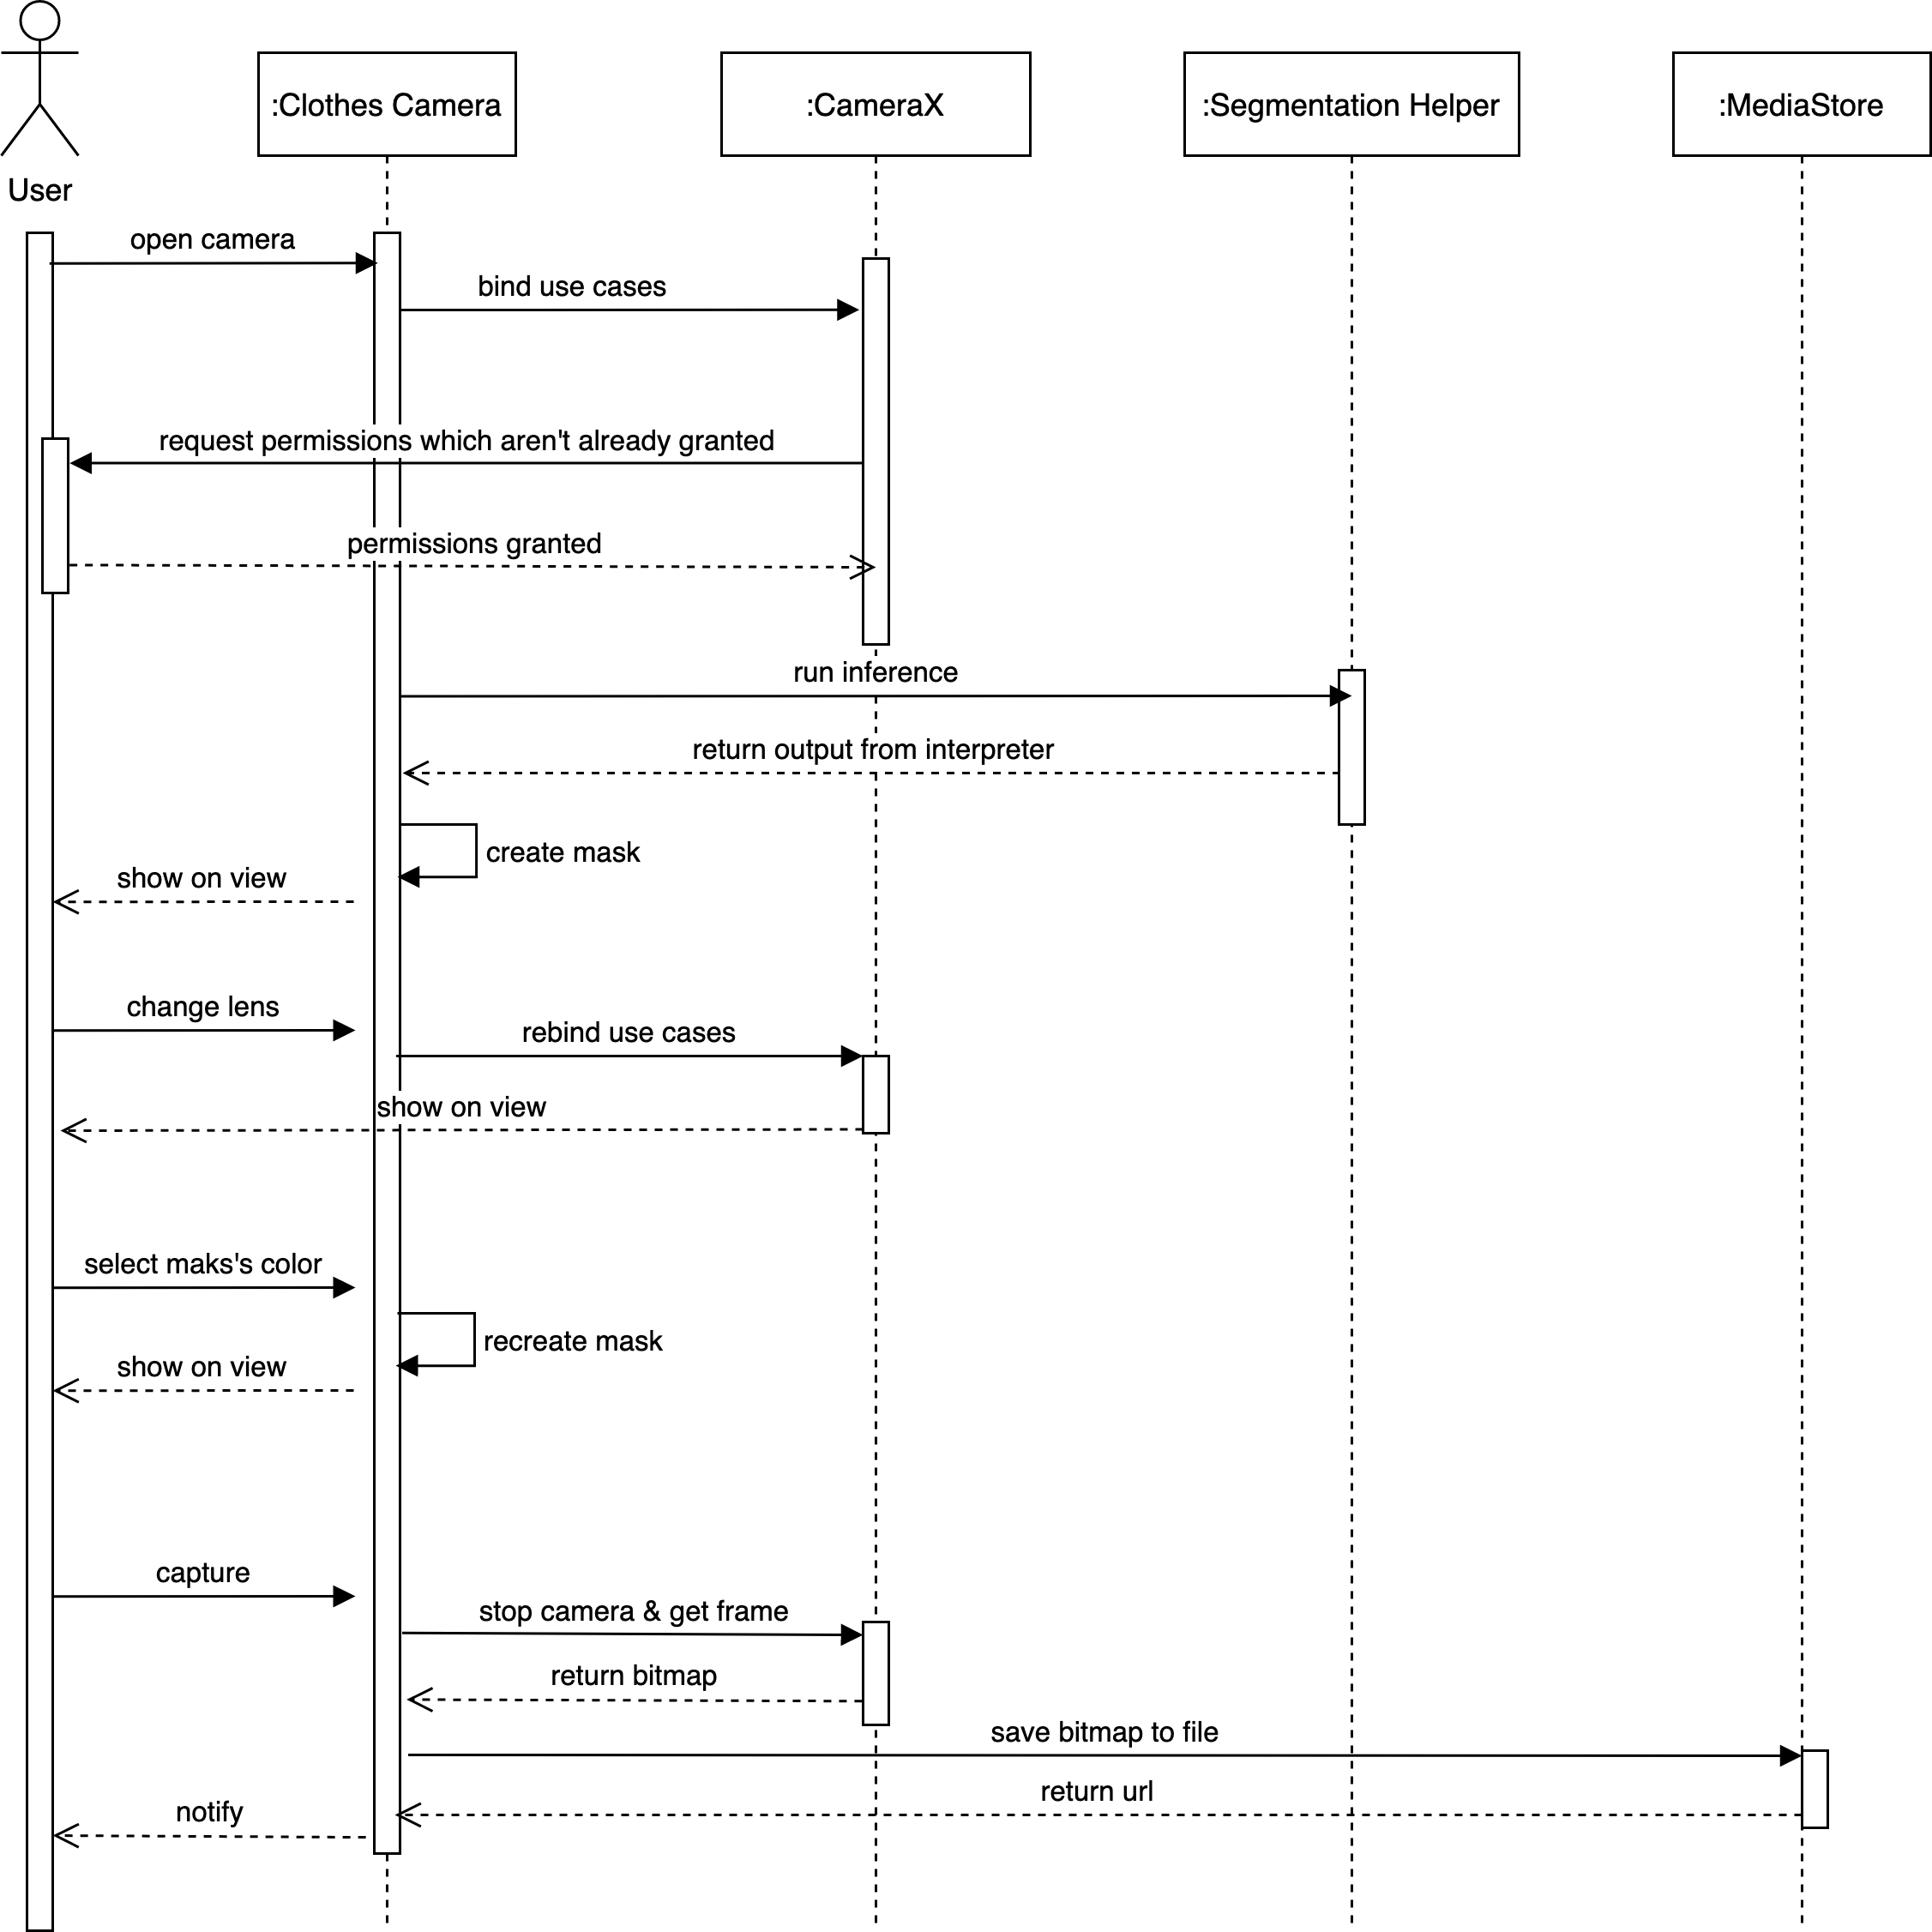
\includegraphics[width=1.0\textwidth]{chapter3/image/clothescamera.png}
    \caption{Sequence diagram for Clothes Camera use case}
    \label{fig:my_label}
\end{figure}

\begin{figure}[H]
    \centering
    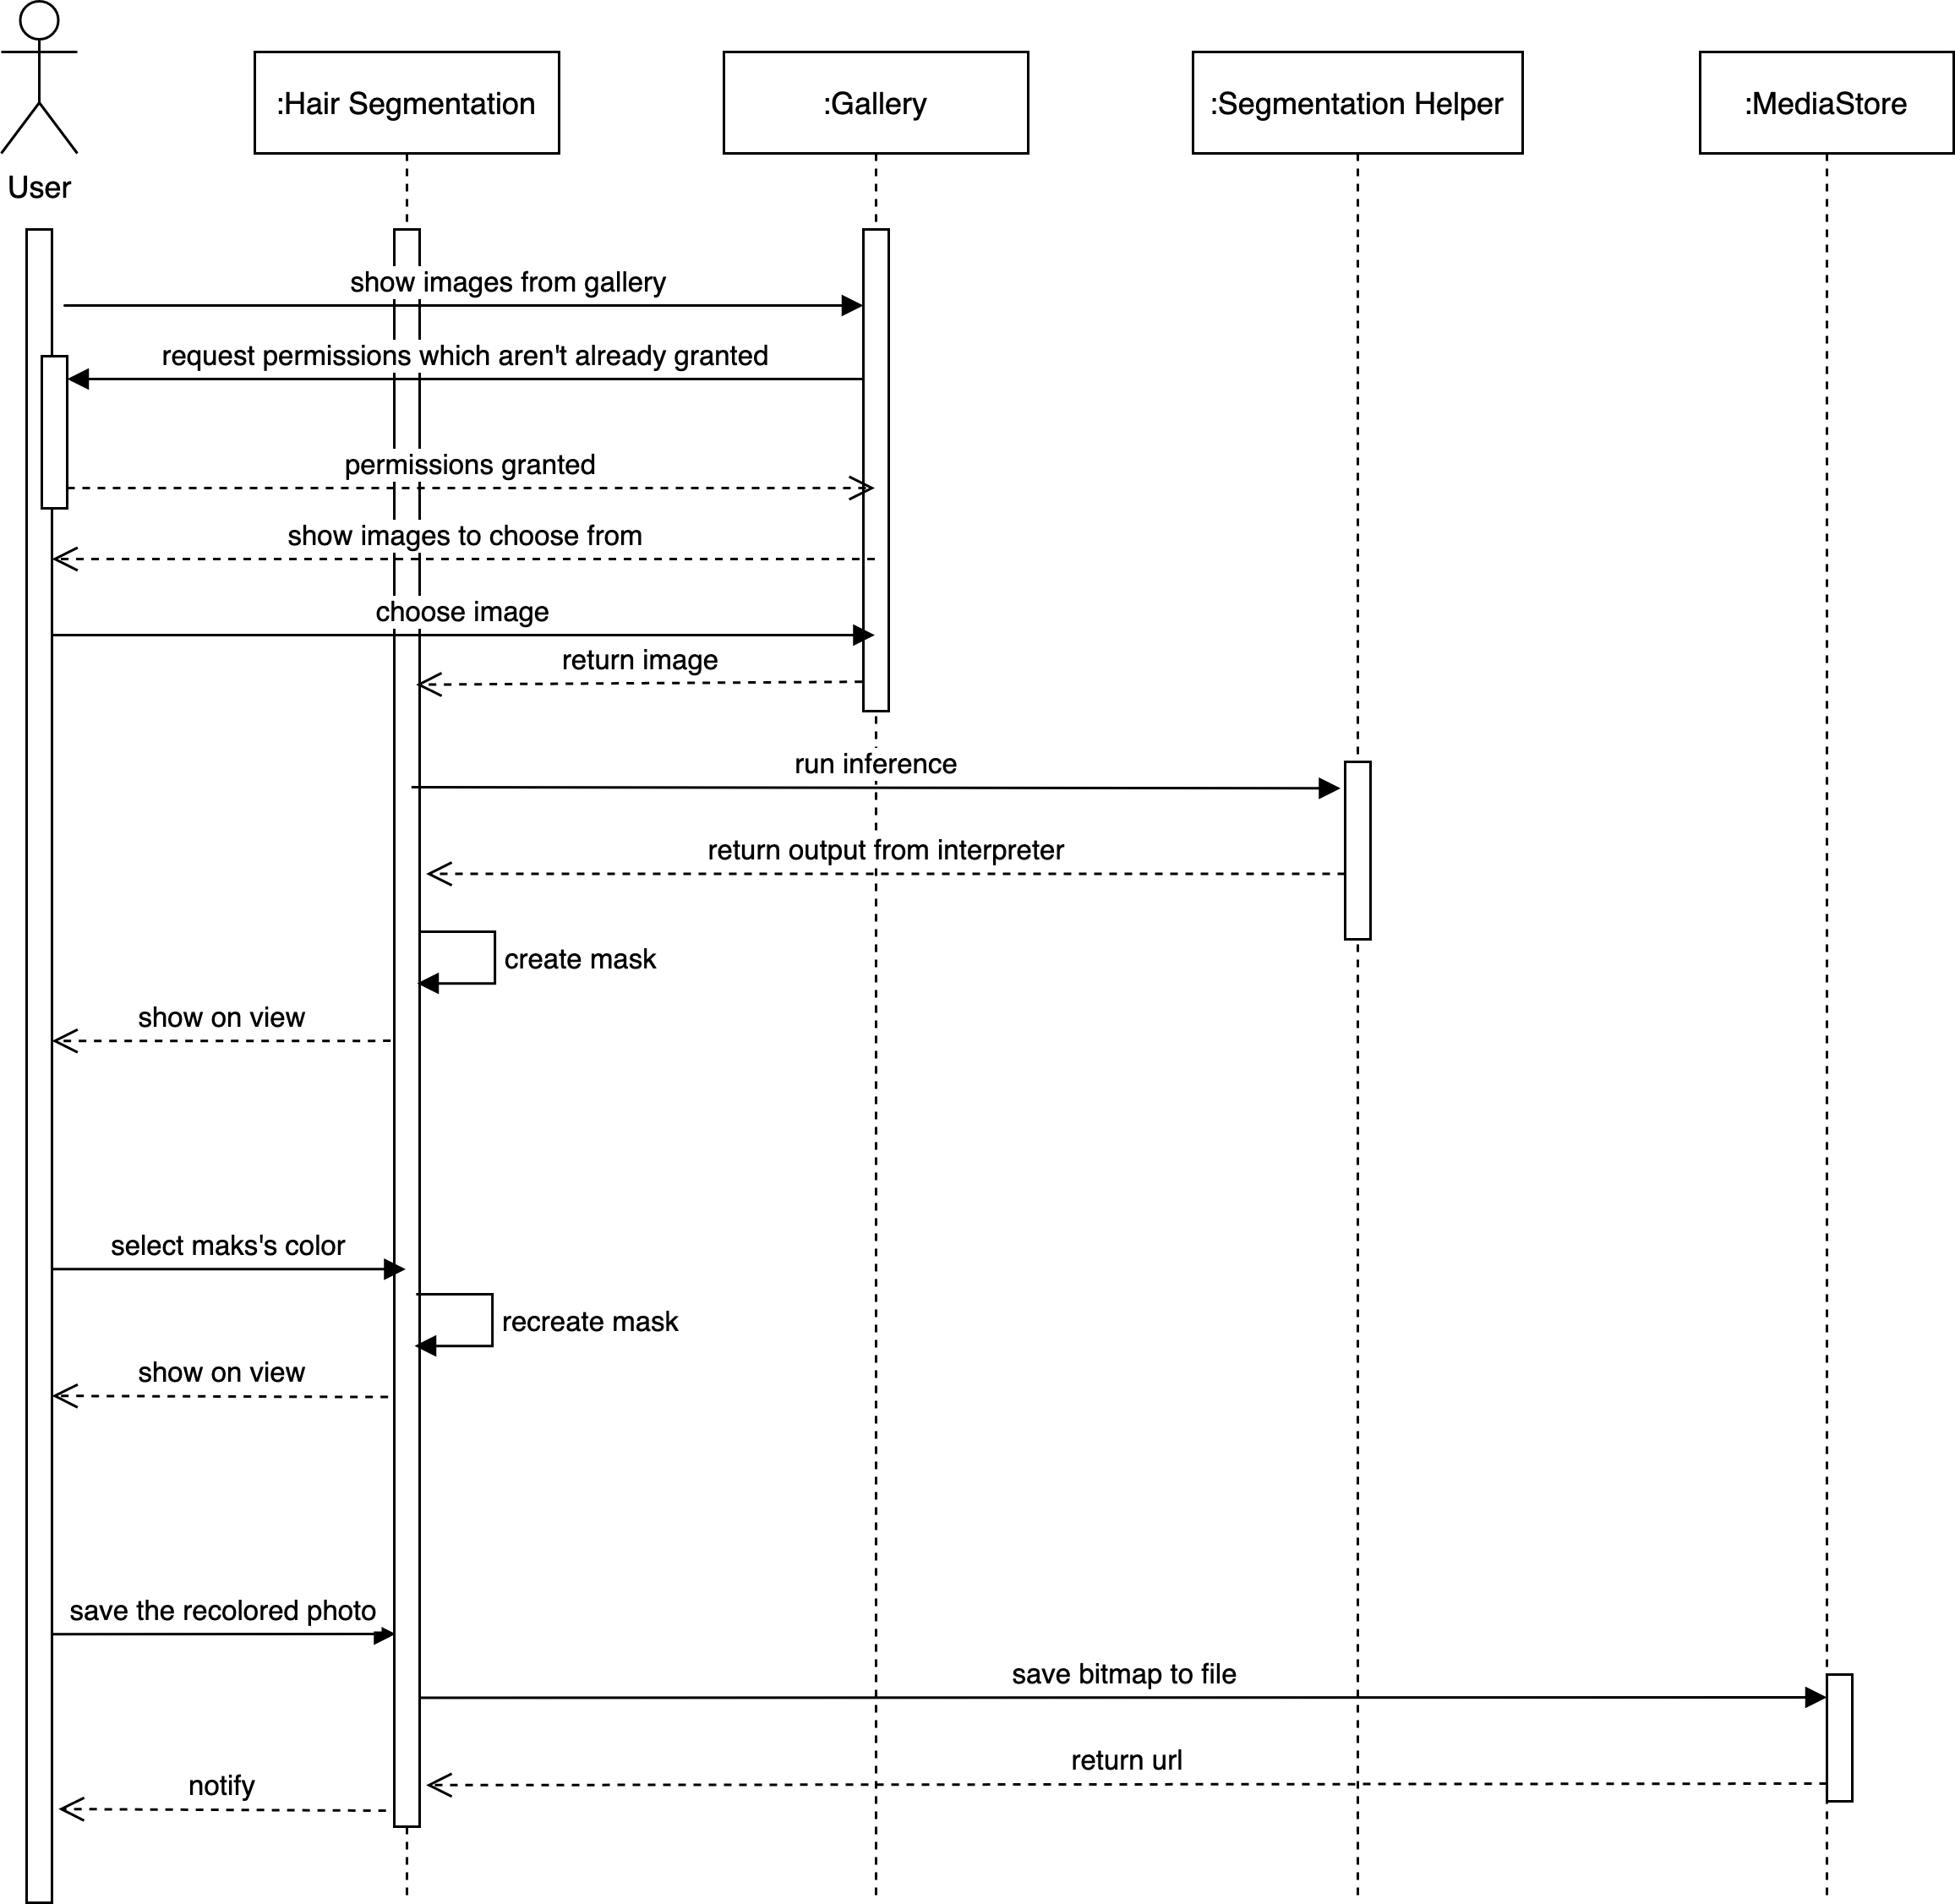
\includegraphics[width=1.0\textwidth]{chapter3/image/hairsegmentation.png}
    \caption{Sequence diagram for Hair Segmentation use case}
    \label{fig:my_label}
\end{figure}
 % 3
\section{Proposed model} \label{sec:model}

Image segmentation models play a vital role in the project and determine the beauty app's latency and user experience. In this section, the proposed CNN is explained, its architecture is about to discuss in more depth. As mentioned previously, as a subset of machine learning, Deep Learning has been showing its accuracy practically in many tasks, such as object detection, object tracking, and object classification. Image segmentation models output a pixel-wise mask of the input image, which is considered as an object segment in the image. Although many DNNs are successful in the image segmentation task in the literature, such as DeepLabV3+ \cite{deeplabv3plus}, PSPNet \cite{pspnet}, they fail to acquire a low latency inference due to their complex architecture in aim to acquire the best accuracy. Considering the requirements, after surveying, I choose U-Net \cite{unet} architecture with MobileNetv2 \cite{mobilenetv2} as a base network for the segmentation tasks. In the following, we dive into the proposed CNN and adaptations to work.
 
 \subsection{MobileNetv2 blackbone}
 MobileNet1 and MobiNetv2 are the first and the second versions in a group of small, low-latency, low-power DNNs named MobileNets. MobileNets is a family of lightweight and general models researched by Google. These models are intended to run with low computational power, such as smartphones, embedded, or IoT devices. Since 2018, when the first version was roll out, there are now three versions with significant improvements after each release. \par
 
 \paragraph{MobiNetv1}
 In MobilNetv1, a key convolution operator called Depth-wise Separable Convolution is first introduced; it takes approximately 70\% less in the number of parameters but only a decrease of 2\% in final accuracy when compared to standard convolution. The basic idea is to replace a full convolutional operator with a factorized one that splits convolution into two separate layers. \par
 
 \begin{figure}[H]
     \centering
     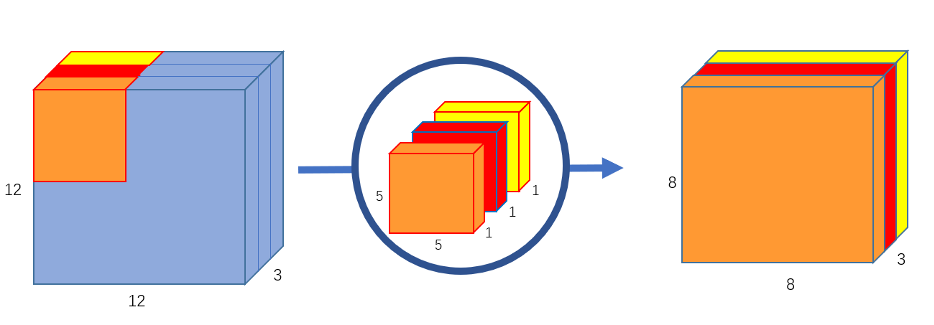
\includegraphics[width=0.9\textwidth]{chapter2/image/mobi1.png}
     \caption{Depthwise convolution, uses 3 kernels (size 5x5) to transform a 12x12x3 image to 8x8x3 image}
     \label{fig:mobi1}
 \end{figure}
 
 \begin{figure}[H]
     \centering
     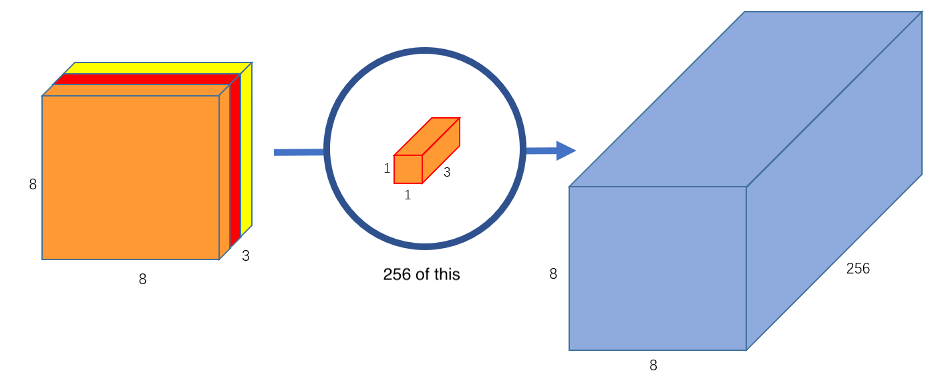
\includegraphics[width=0.9\textwidth]{chapter2/image/mobi2.png}
     \caption{Pointwise convolution, transforms an image of 3 channels (size 8x8x3) to an image of 256 channel (size 8x8x256)}
     \label{fig:mobi2}
 \end{figure}
 
 The entire process can be divvied into two steps: Depthwise convolution and Pointwise convolution. At first, a single-depth convolution is separately applied to each channel of the previous feature map. Take the previous feature map with three channels, illustrated in \textbf{Figure \ref{fig:mobi1}}, Depthwise convolution would consist of three kernels, and each kernel would iterate one channel of the feature map. As the convolutional operations have a single depth, the output has the depth remained the same. Second, N number of Point-wise convolutions are used to combine the outputs of the depth-wise convolution, where N is the desired channel depth of the resulting feature map. In the case of \textbf{Figure \ref{fig:mobi2}}, N is equal to 256. 
 
 \paragraph{MobiNetv2}
 MobileNetV2 is introduced in CVPR 2018, regarded as the next generation of mobile model. It inherits Depthwise Sepratable convolution from MobileNetv1. Although built upon the ideals of MobilNetv1, MobileNetv2 proposes two significant changes to the architecture: linear bottlenecks layers and shortcut connections between the bottlenecks. The basic structure of a bottleneck residual block is shown in \textbf{Figure \ref{fig:mobi2bottleneck}}. \par
 
 \begin{figure}[H]
     \centering
     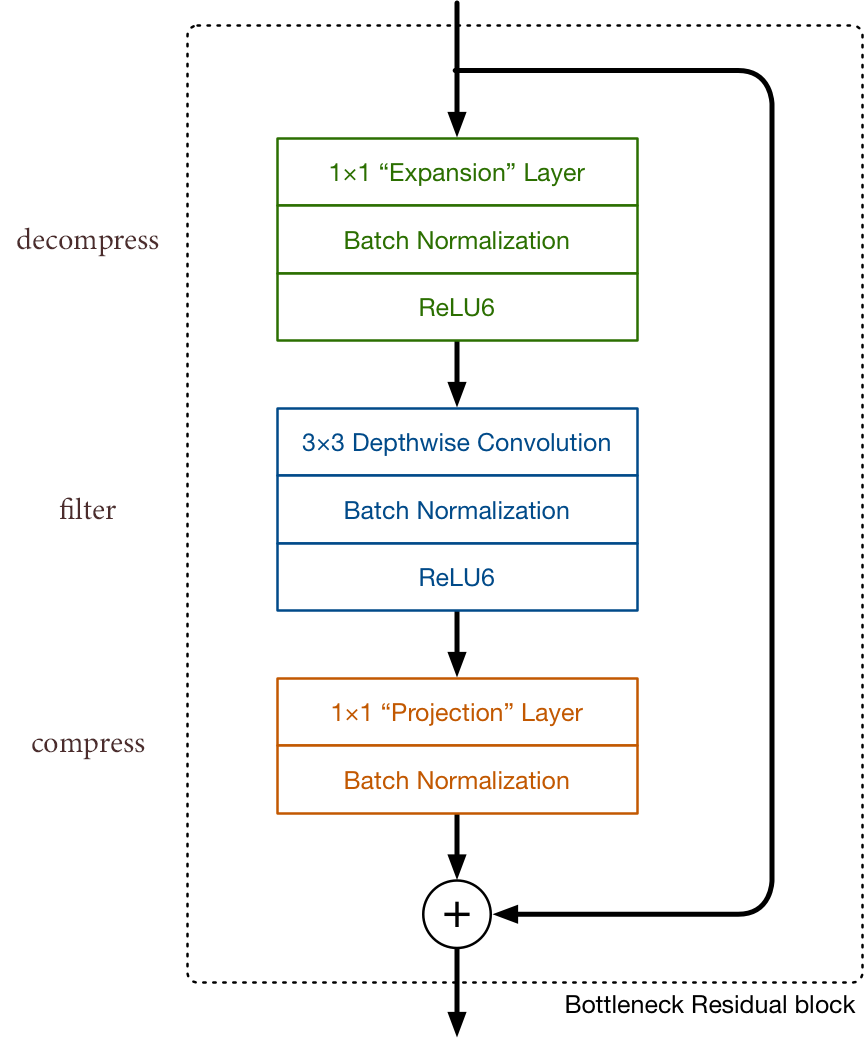
\includegraphics[width=0.6\textwidth]{chapter3/image/block_edited.png}
     \caption{A bottleneck residual block.}
     \label{fig:mobi2bottleneck}
 \end{figure}
There are three convolutional layers in this building block. The first layer is a 1x1 pointwise convolution which is similar to in MobileNetv1.  Its purpose is to expand the number of channels in the data before it goes into the 3x3 depthwise convolution. This expansion layer plays a role as a decompressor that restores the data to its full form. On the other hand, the last convolutional layer, which is also called a bottleneck layer, is a 1x1 pointwise convolution. However, this layer makes the number of channels smaller; in fact, it contrasts to in MobileNetv1 where the pointwise convolution either kept the number of channels the same or doubled them. Its purpose is to projects data with a high number of dimensions (channels) into a tensor with a much lower number of dimensions. In other words, the projection layer compresses the data to make it small again. As a result, the input and the output of the block are low-dimensional tensors, while the filtering step that happens in between is done on a high-dimensional tensor.
 \par
 
 One small change is that the activation function used by MobineNetv2 is ReLU6:
 \begin{equation}
 y = ReLU6(x) = min(max(0, x), 6)
 \end{equation}
 This is like the traditional ReLU as a non-linearity, but it prevents activations from becoming too big. The reason for this is that ReLU6 is more robust than regular ReLU when using low-precision computation. Moreover, the shape of this function is similar to the shape of a sigmoid function. \par
 
 
 I integrate MobinetNetv2 into the overall network excluded the top, which consists of fully-connected layers; otherwise, the image input must be 224x224. MobileNetv2 works as a feature extractor for a second neural network. It is remarked that MobileNetv2 has a good balance between the used resources (memory and FLOPS) and accuracy trade-off. This backbone is far better among other lightweight base networks, such as MnasNet \cite{mnasnet}, SqueezeNet \cite{squeezenet}.
 
 
 \subsection{U-Net architecture} \label{sec:unet}
 This section describes the proposed network entirely. The network is based on the general-purpose U-Net architecture in order to accommodate hair and clothes segmentation tasks. \par
 
 \begin{figure} [H]
     \centering
     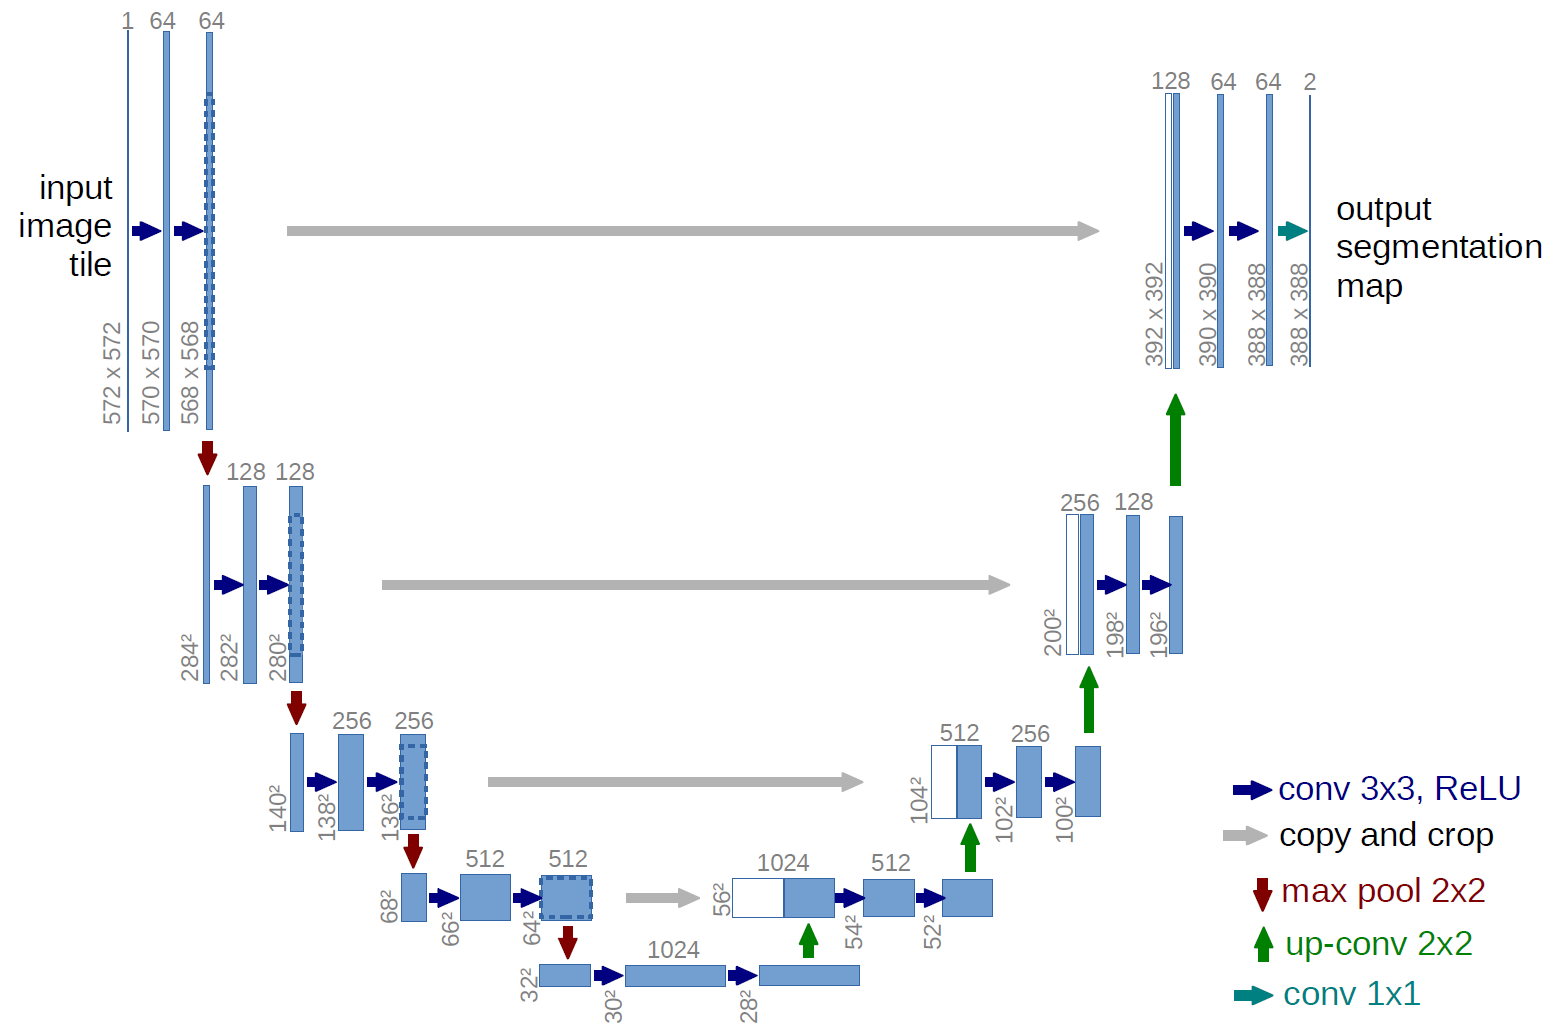
\includegraphics[width=0.7\textwidth]{chapter3/image/u-net.png}
     \caption{Illustration for U-shaped architecture in the origin paper \cite{unet}.}
     \label{fig:unet1}
 \end{figure}
 
 U-Net is an autoencoder type network architecture introduced in \cite{unet} for semantic segmentation of biomedical images in 2015. However, U-Net achieves high accuracy in other segmentation tasks as well. It introduces skip-connections to the autoencoder architecture to improve resolving and propagating higher-level features in the decoder block.
As a consequence, the decoder can access information from the encoder, such as edges, corners and angles in the original images. Many semantic segmentation networks utilize this ideal where information from the encoder is passed to the decoder via long skip-connections to preserve higher-level information found at higher resolutions in the encoder. \par

\vspace{5mm}

 \begin{figure} [H]
     \centering
     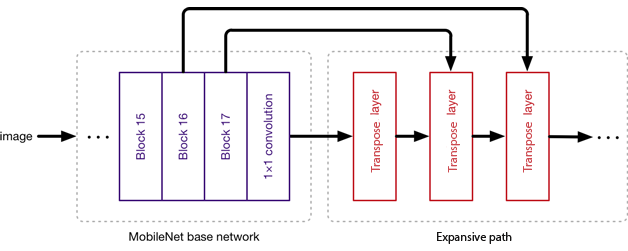
\includegraphics[width=0.9\textwidth]{chapter3/image/architec.png}
     \caption{UNet architecture with the MobileNetv2 base model.}
     \label{fig:unet2}
 \end{figure}
 
 While \textbf{Figure \ref{fig:unet1}} depicts the origin U-Net architecture in view of layers, \textbf{Figure \ref{fig:unet2}} shows the adapted network in view of components. More specifically, the contracting path replicates the architecture of MobileNetv2 with 17 blocks in total. On the other hand, the expansive path consists of an upsampling of feature maps followed by a 2x2 convolution that halves the number of feature channels. The upsampling method is transposed convolutions. The number of max-pooling layers 
 equal to the number of transposed convolutions and equals five. Generally, the proposed network has the same architecture as the original version; however, I made slight modifications.
 The first adaptation I made is that batch normalization is only used in the contracting path of the network. It changes results from preliminary experiments and increases the speed of the network without decreasing the accuracy. The second adaptation lies at the two last layers, where the last convolution has a kernel size of one and is followed by a softmax activation. As a result, the network would output a final probability map, which represents the desired mask. Following that, the loss is calculated as a binary cross-entropy function on a pixel-wise basis.
 \par % 3


\section{App Development}  \label{androidapp}
In previous section, DNN for hair and clothes segmentation has been reviewed. In this section, proposed solution to the task of intergrating the model into the Android app is demonstrated. Consequently, the implementation of an Android app is rather easy once you have a proper design and well-defined solutions. 
\subsection{Pipeline}
One of the most important use cases of common beauty or augmented reality applications is real-time camera visuality. In case of the thesis, the beauty app has two instance of these use cases: \emph{Hair Camera} and \emph{Clothes Camera}. Indeed, they are addressed as the most intricate work in the app. To clear it up, I proposed a pipeline used for both the two use cases, however the proposed pipeline is so general that can be reused in other applications.  

\vspace{3mm}
\begin{figure} [H]
    \centering
    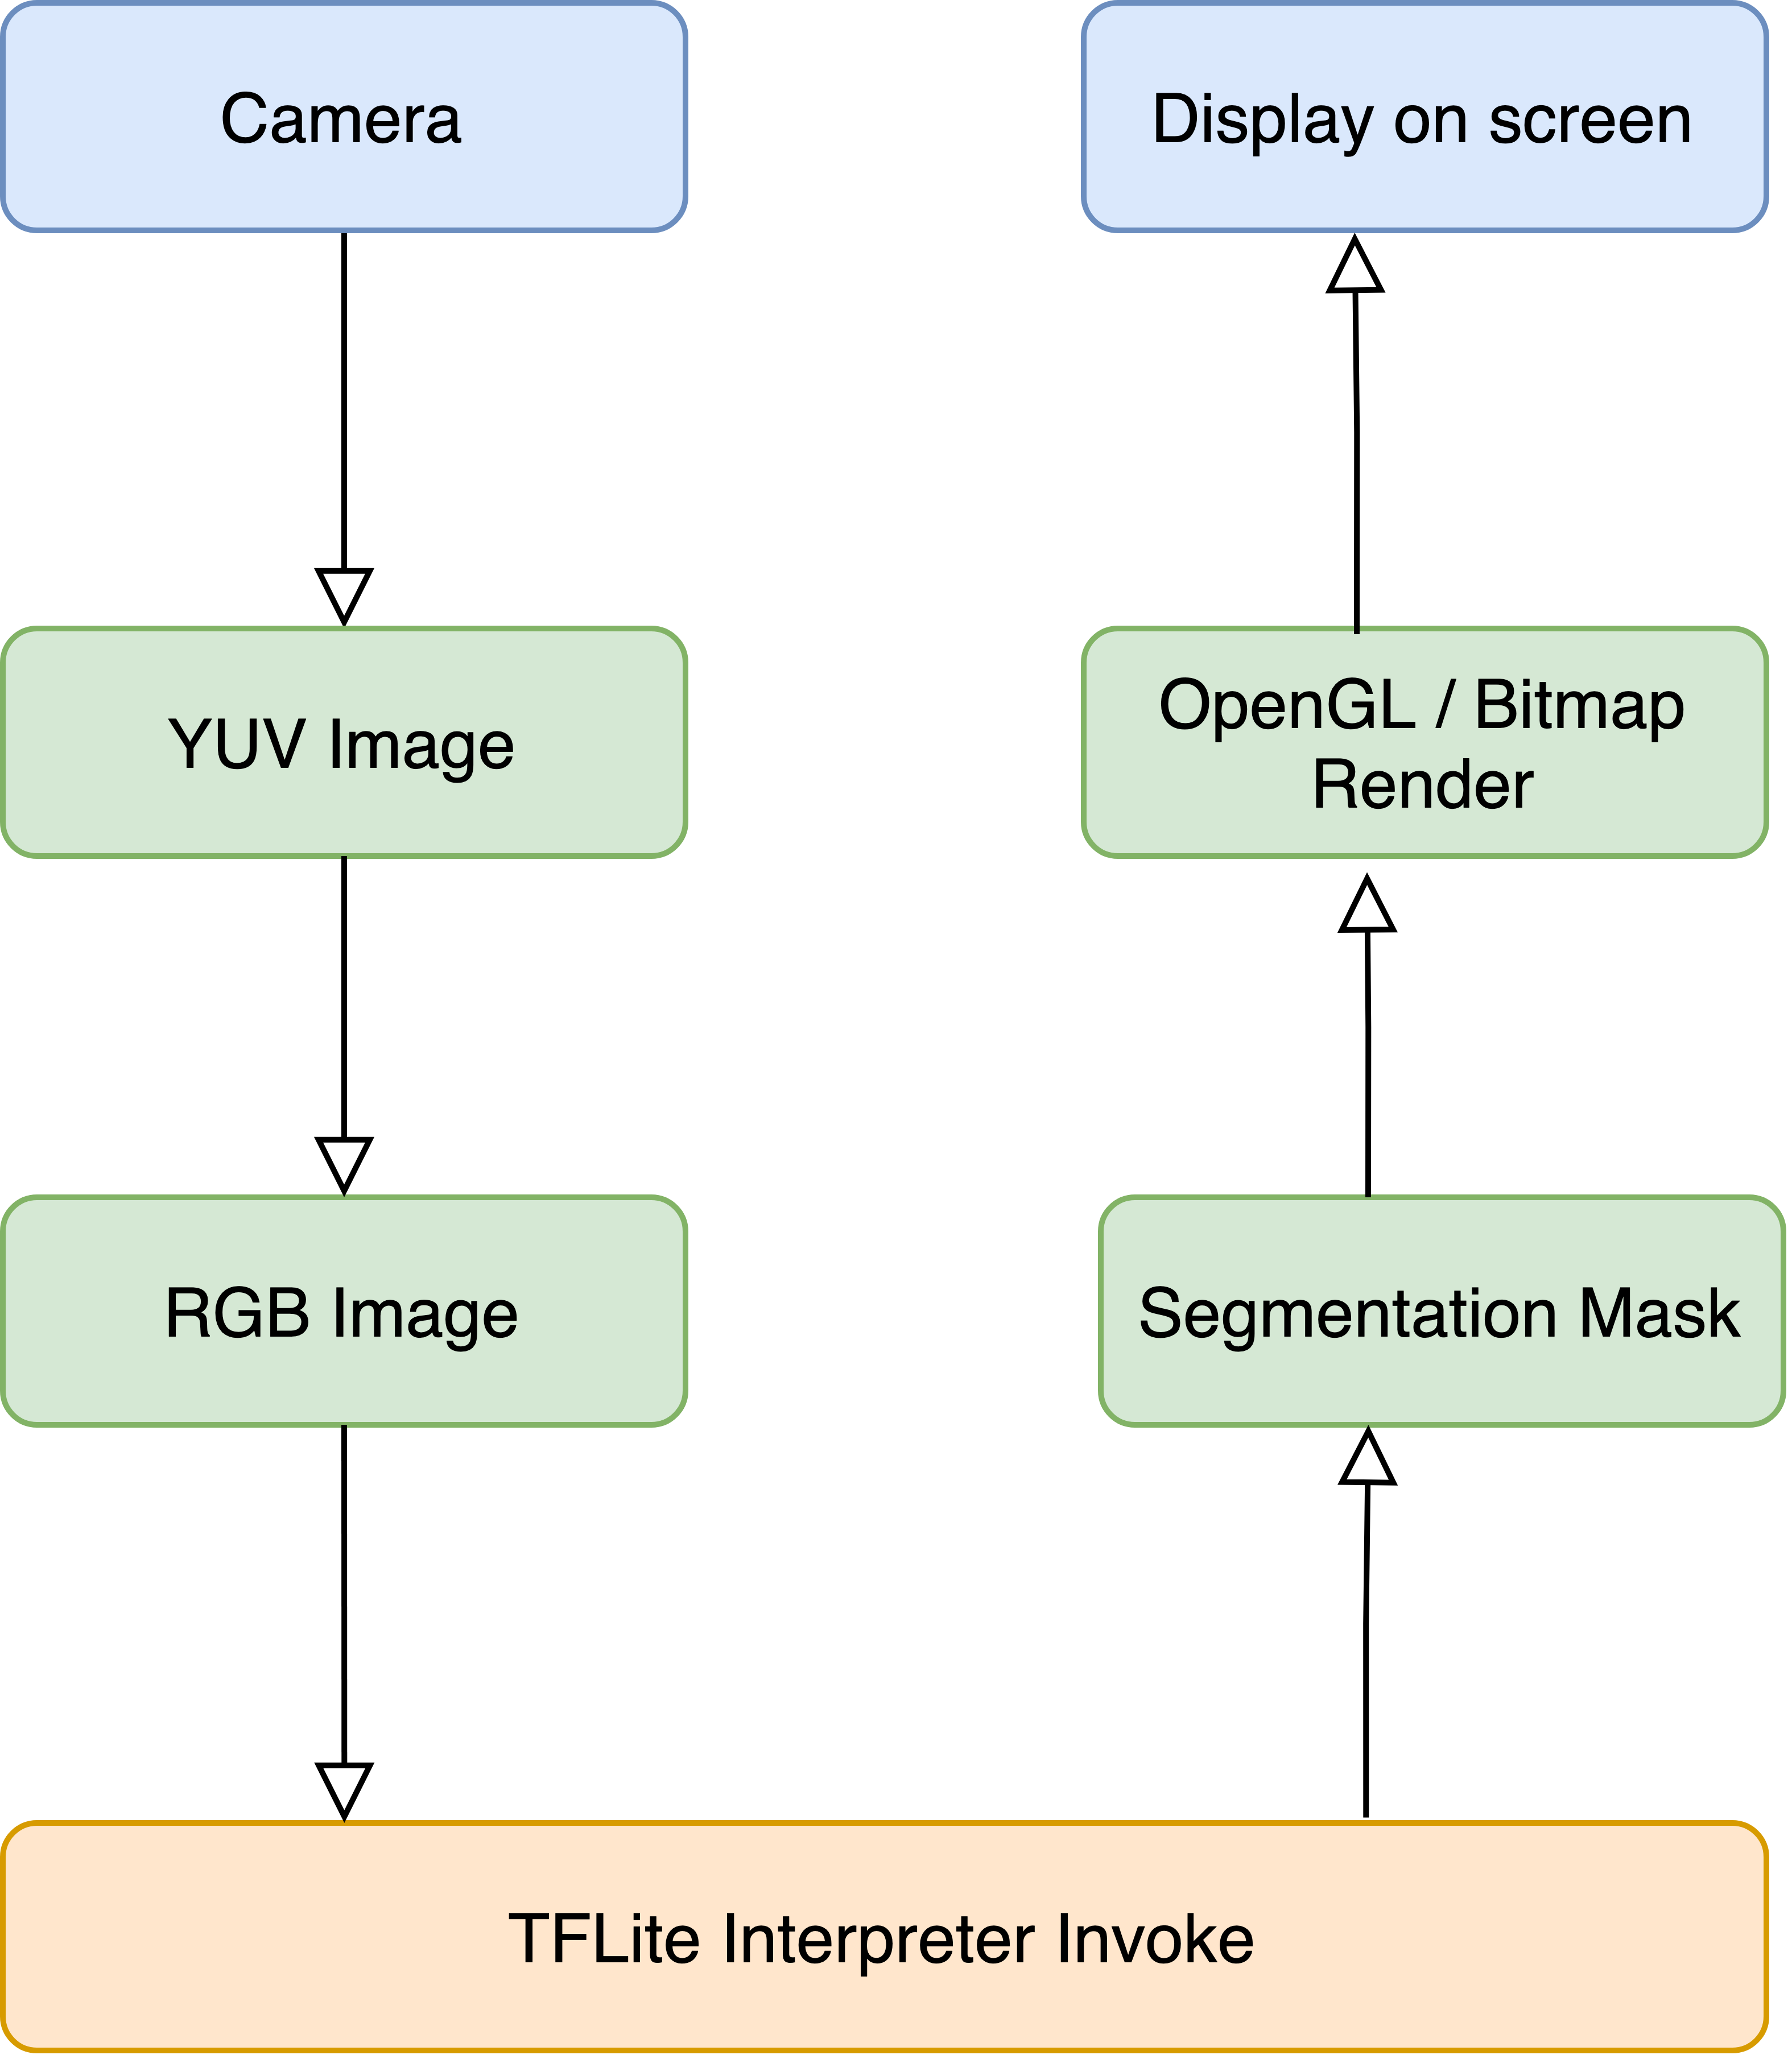
\includegraphics[width=0.6\textwidth]{chapter3/image/apppipeline.png}
    \caption{Pipeline for camera use case}
    \label{fig:my_label}
\end{figure}
 
The pipeline starts with receiving data from hardware, here is the camera lens. CameraX library, which is mention in \textbf{section \ref{sec:camerax}}, supports entire this work.  However, each camera framework outputs image under a different format. For example, if app uses CameraX or Camera2 API, output images are in YUV\_420\_888 format. If app uses Camera API, output images are in NV21 format. After that, the image is converted to a RGB image and represented as byte buffer in order to feed to the model. Subsequently, the TFLite interpreter, which is situated in middle, receives input buffer and outputs the result buffer of the model. The buffer is then preprocessed before being rendered. Finally, the mask is displayed on screen, as a result, the camera view is overlaid with the mask.

 
\subsection{On-device inference}

Making an inference involves taking single or multiple inputs (images, text, video) and pushing them through the many layers of the network. In matters of making on-device predictions, it is vital to have a general understanding of hardware types where the model runs. Almost all smartphones have both CPUs and GPUs. In Android, there are even a few libraries that work with these hardware platforms in order to supply accelerators for deep learning.  \par

Android Neural Networks API (NNAPI) is one of them, which is available for Android 8.1 and above. NNAPI is a machine learning library that supports a wide variety of chipsets, including Snapdragon. There are three options for hardware accelerators, namely GPU, NNAPI, and CPU. Technically, NNAPI is an Android C API designed for executing computationally intensive operations for machine learning on Android devices. NNAPI runtime is a shared library that situated between an app and backend drives, enables NNAPI to run on multiple mobile platforms (Snapdragon, AMD...) \par
 \begin{figure} [H]
     \centering
     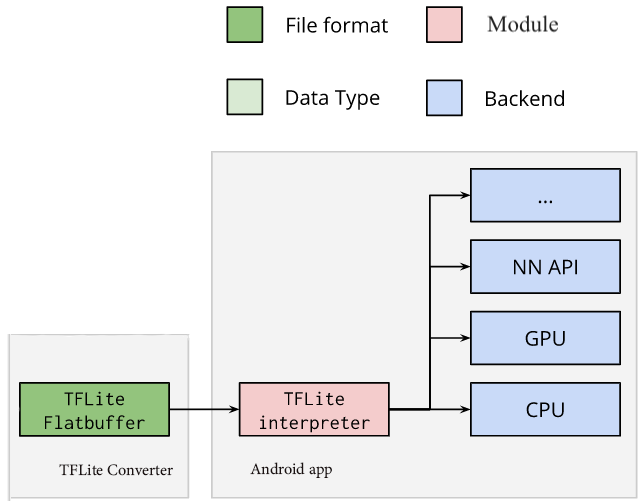
\includegraphics[width=0.7\textwidth]{chapter3/image/client pipleline_edited.png}
     \caption{Workflow of TFLite library for Android}
     \label{fig:my_label}
 \end{figure}
Built upon this, TFLite Interpreter in Android develops both NNAPI delegate and GPU delegate. The GPU delegate is optimized to run 32-bit and 16-bit float-based models where a GPU is available. Although the GPU delegate is well-run and supports more operating systems, I find the NNAPI delegate more effective and battery saving. The following is the code used for preparing input data and run inference with TFLite:\par 
\vspace{5mm}

\begin{lstlisting}[ caption=NNAPI Inference implementation]
// Image pre-processing before feeding into the DNN
private val tfImageProcessor by lazy {
    val cropSize = minOf(bitmapBuffer.width, bitmapBuffer.height)
    ImageProcessor.Builder()
        .add(ResizeWithCropOrPadOp(cropSize, cropSize))
        .add(ResizeOp(
            tfInputSize.height, tfInputSize.width,
            ResizeOp.ResizeMethod.BILINEAR))
        .add(Rot90Op(-imageRotationDegrees / 90))
        .add(NormalizeOp(127.5f, 127.5f))
        .build()
}

// Initialize interpreter with GPU delegate
private val tflite by lazy {
    Interpreter(
        FileUtil.loadMappedFile(this, MODEL_PATH),
        Interpreter.Options().addDelegate(NnApiDelegate())
    )
}

val output =  tflite.run(tfImageProcessor.process(input))
\end{lstlisting}
 
 
 
 
 
 
 
\subsection{Rendering masks}
After semantic information is obtained from the interpreter, segmentation maps are generated. In order to format and display them, two methods of rendering are proposed, namely Bitmap and OpenGL.

\subsubsection{Bitmap}
A bitmap is simply a rectangle of pixels. Each pixel can be set to a given color but exactly what color depends on the type of the pixel. A so-called type of pixels is \emph{ARGB\_8888} where a pixel has four channels (Alpha, Red, Green, Blue) and allocates each eight bits of storage.\par

Bitmap is the first rendering method applied to the app because its well-support in Android API. In fact, Bitmap is a popular 2D graphics class, and Android allows you to use the \emph{Bitmap} class for working with bitmaps. It extends from \emph{Drawable} class which is a general and abstract class for something that can be drawn.  \par


\begin{lstlisting}[caption=Bitmap rendering implementation]
val mask = Bitmap.createScaledBitmap(output, screen.width, screen.height)

overlay.setImageBitmap(
    mask
)
\end{lstlisting}

It would be effective if you do not modify bitmaps too often, because every time you change the content of a bitmap, it is uploaded again as a GPU texture the next time you draw it. As a result, there would have a delay. \par

\subsubsection{OpenGL ES}
OpenGL is a well-used open-source graphic library for rendering 2D and 3D vector graphics on almost all platforms. Android OS is not an exception; it uses a subset of OpenGL’s API called OpenGL for Embedded System (OpenGL ES). OpenGL ES is cross-platform, albeit closed-source. In Android, OpenGL ES is loaded to NDK as a shared library, and SDK wraps it up for ease of implementation.
\par

\begin{figure} [H]
    \centering
    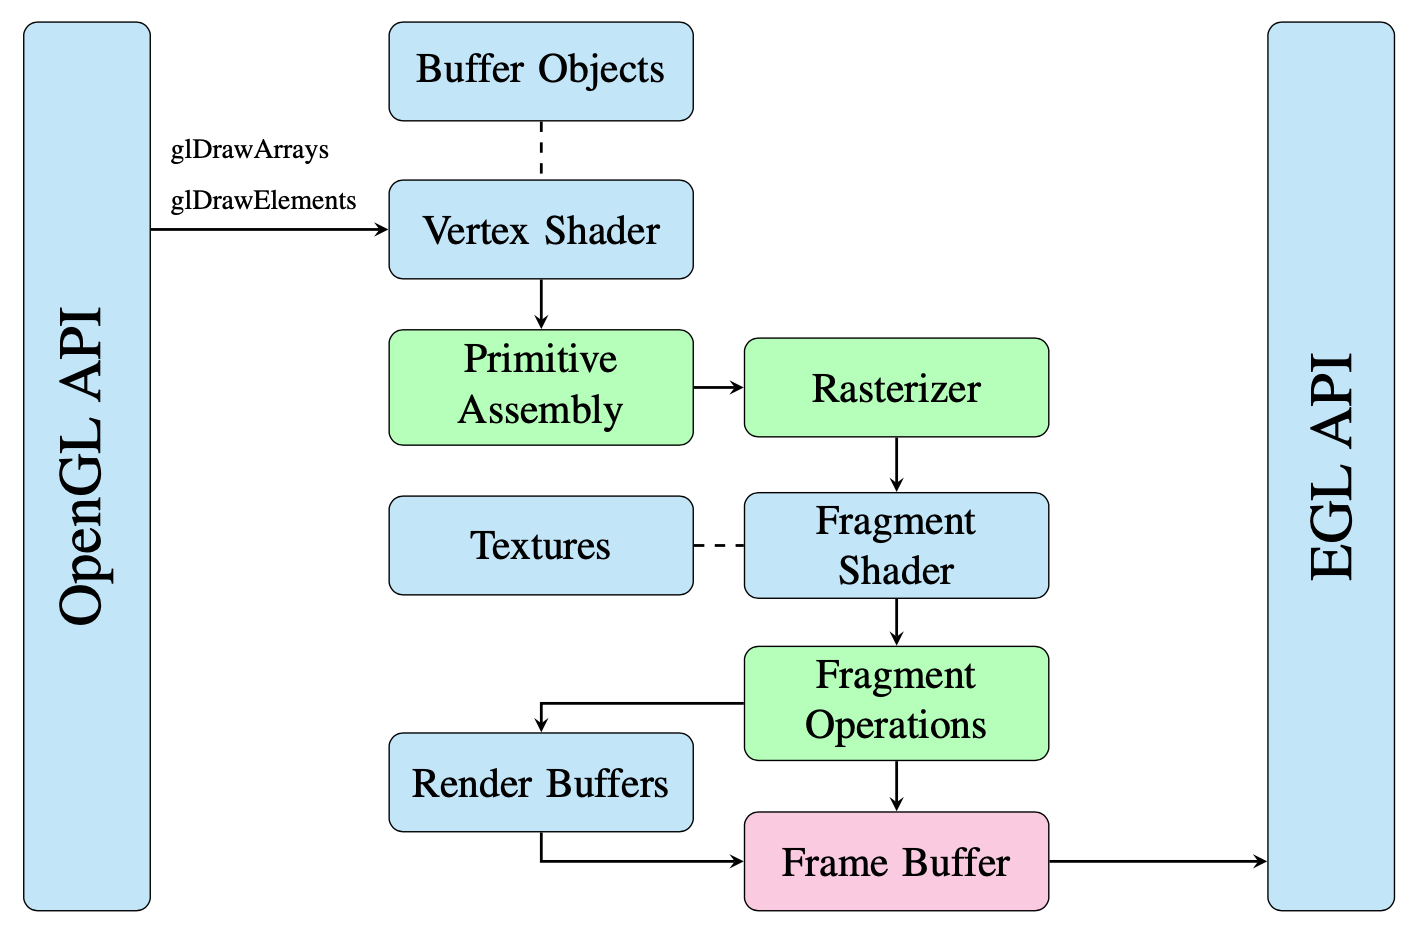
\includegraphics[width=0.7\textwidth]{chapter3/image/openglpipeline.png}
    \caption{OpenGL ES 2.x pipeline. Blue node: You have to set, Green node: You do not have any control, Magenta node: Optional. Source: \cite{openglpipeline}.}
    \label{fig:coordinates}
\end{figure}

The first step in the rendering process is sending the vertices and the texture positions along with the textures, as shown in \textbf{Figure \ref{fig:coordinates}}. To do so, the points that were passed to the renderer first combined into a 1-dimensional array of (x,y,z) values, then uploaded to the vertex shader along with the corresponding texture coordinates of the segmentation mask. These values fall into the range of [−1, 1] in the GLES coordinates, where the point (0, 0) being the middle of the screen. However, the texture coordinates are ranged from [0, 1] where point (0, 0) being the bottom left corner. After the coordinate is uploaded to the vertex shader, the textures are sent to the fragment shader. In the implementation, it was found that it is more efficient to load the whole mask's texture before starting the drawing loop.\par



%We send two different textures to the shader. The segmentation mask which consists of one channel and the color image of the original scene to perform the inpainting in the fragment shader. These textures are sent after the segmentation mask is generated and the hit test is performed by using GLES interface function glTexImage2D. \par

 % 3

\setcounter{figure}{0}
\mychapter{4}{CHAPTER 4. EXPERIMENTS AND RESULTS}\label{ch:chap4} 
% 10 trang\

In this chapter, the thesis presents experiments and evaluates the method proposed in the previous chapter. Before going into a detailed evaluation, the benchmark dataset is briefly introduced. Concretely, \textbf{section \ref{sec:dataset}} describes three datasets which are used for model training and testing, consisting of two datasets for the hair segmentation task and one dataset for the clothes segmentation task. After that, \textbf{section \ref{sec:experiments}} describe the process of training the model in detail. Finally, \textbf{section \ref{sec:results}} indicates the results of the Android app and the models obtained from the thesis.

\section{Experiments} \label{sec:experiments}
       
\subsection{Datasets} \label{sec:dataset}

\paragraph{DeepFashion2}

\begin{figure} [H]
    \centering
    \captionsetup{justification=centering}
    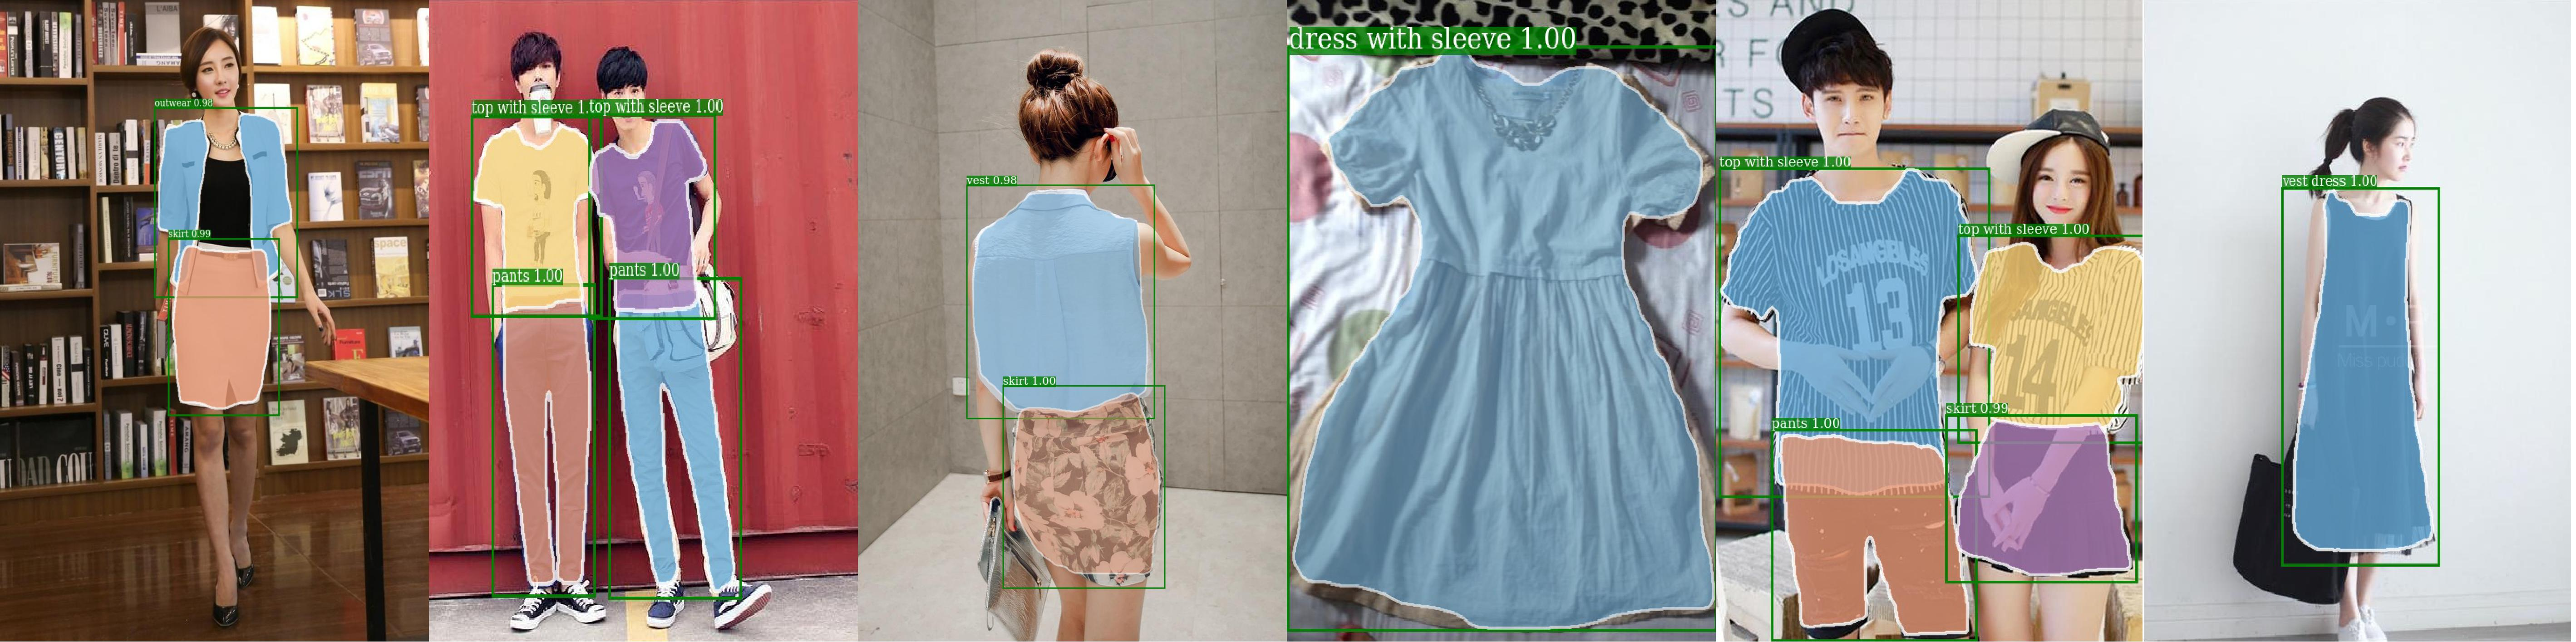
\includegraphics[width=0.9\textwidth]{chapter4/image/deepfashion20.jpg}
    \caption{Polygon annotation examples in DeepFashion2 dataset}
    \label{fig:df}
\end{figure}

DeepFashion is a large-scale clothes dataset with over 800.000 images of 46 clothing categories under different scenarios, namely street snapshot, store. DeepFashion2 is an extension of DeepFashion, proposed to study a broad spectrum of computer vision applications for fashion, including clothes retrieval, clothes recommendation, and virtual try-on. Applied for comprehensive tasks, DeepFashion2 has richer annotations such as style, bounding box, viewpoint, scale, etc. It contains 491.000 images of 13 clothing categories. Here is the identity number and name of the whole thirteen categories: 1 represents short sleeve top, 2 represents long sleeve top, 3 represents short sleeve outwear, 4 represents long sleeve outwear, 5 represents vest, 6 represents sling, 7 represents shorts, 8 represents trousers, 9 represents skirt, 10 represents short sleeve dress, 11 represents long sleeve dress, 12 represents vest dress and 13 represents sling dress. \par 

\begin{figure} [H]
    \centering
    \captionsetup{justification=centering}
    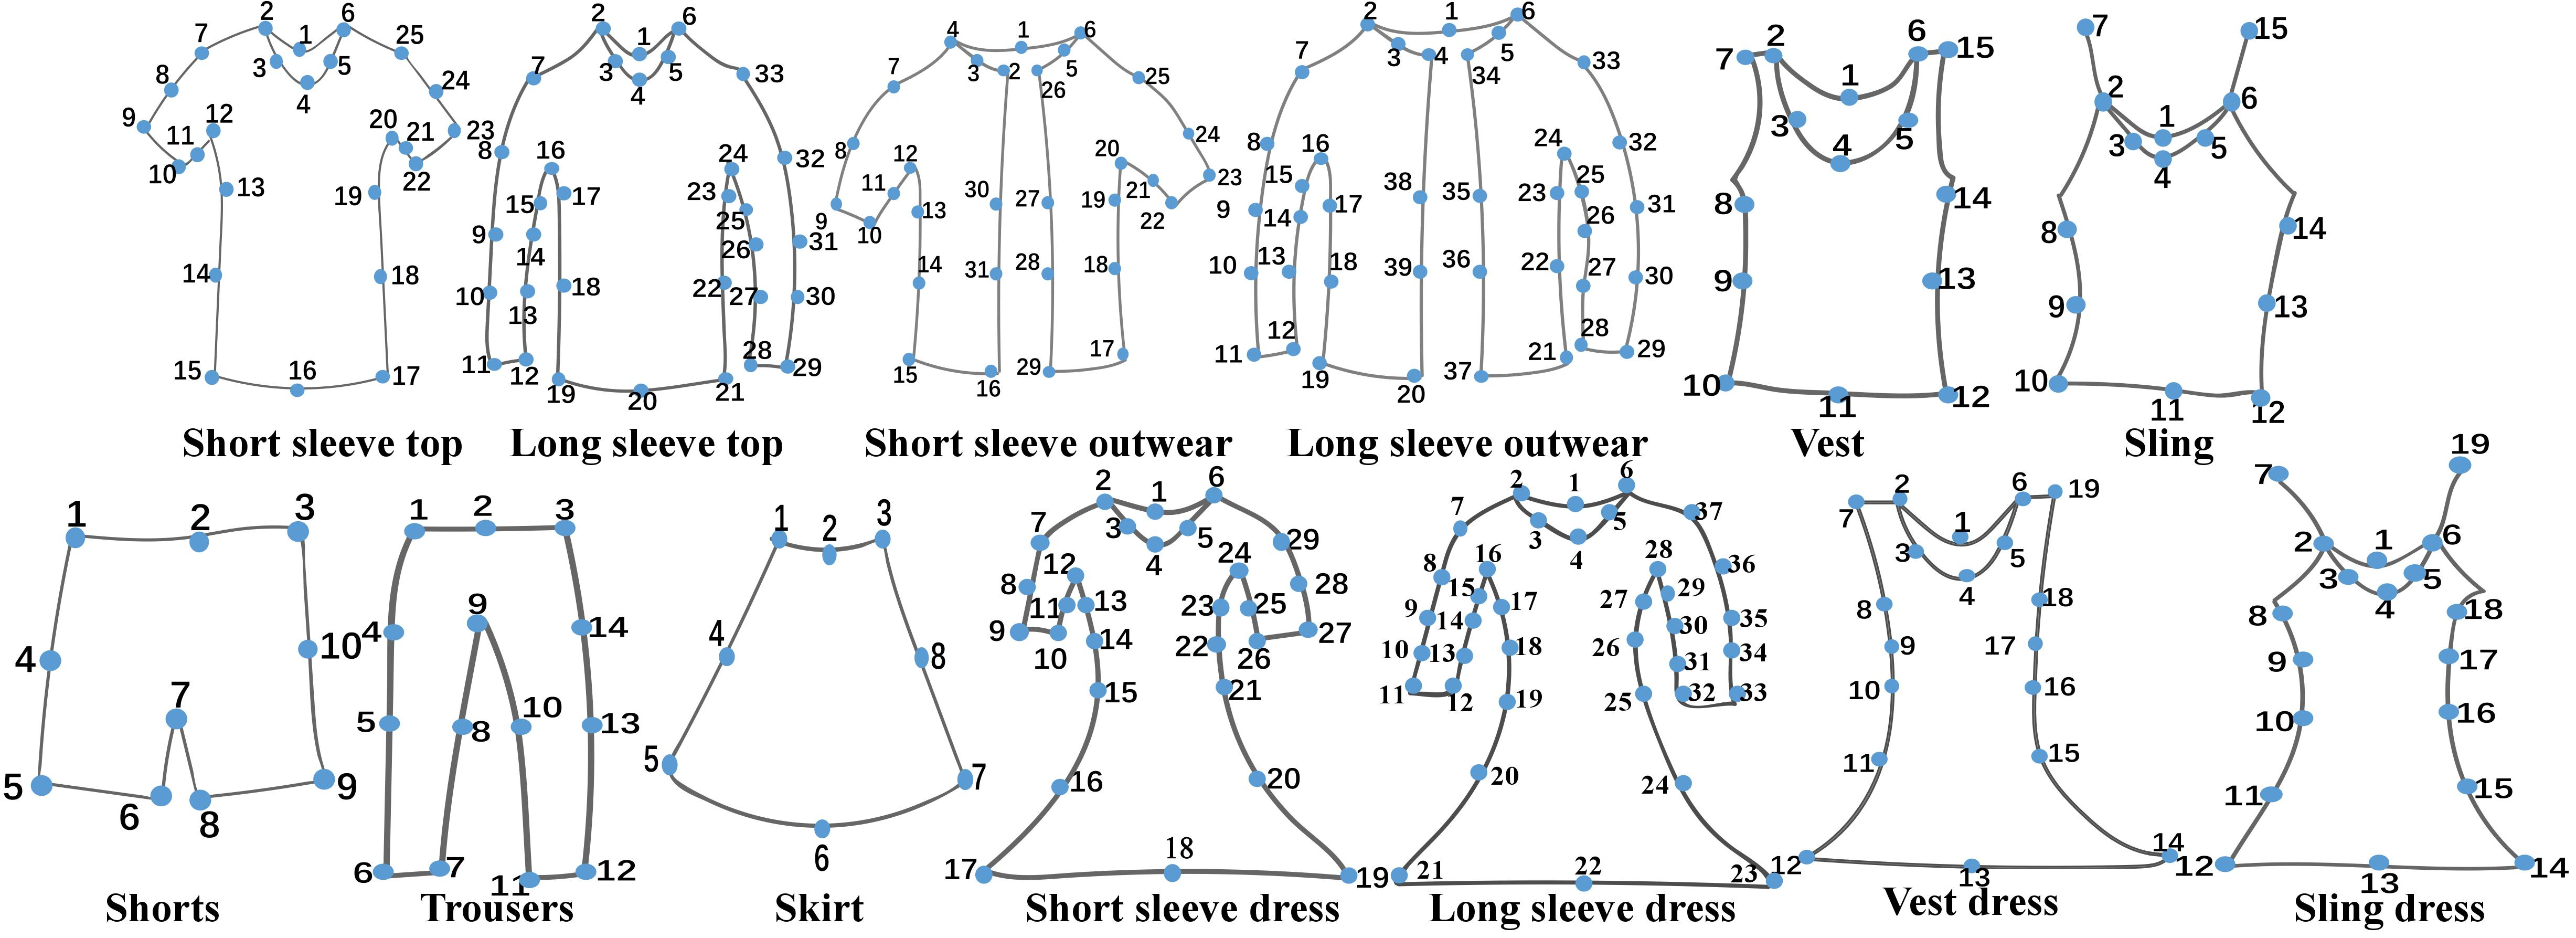
\includegraphics[width=0.9\textwidth]{chapter4/image/deepfahsion2_class.jpg}
    \caption{Thirteen categories of DeepFashion2 dataset}
    \label{fig:dfcate}
\end{figure}

However, I only use the dataset for upper-body clothes (includes the first six categories) recognition. Thus images with categories from 6 to 13 are excluded. After removing lower-body clothes, the dataset remains 137,850 images in the training set. \par


\noindent Differences when compare DeepFashion2 with DeepFashion:
\begin{itemize}
\item DeepFashion2 includes multiple items (pieces of clothing) in an image, while DeepFashion only has a single item per image.
\item DeepFashion is annotated with sparse landmarks per, each piece of cloth only has from 4 to 8 landmarks. In DeepFashion2, each item is manually labeled. With bounding box, mask, dense landmark (20 per item on average)
\item DeepFashion annotations are stored in text files, while DeepFashion2 annotations are stored in JSON format files.
\end{itemize}


\paragraph{Figaro1k}

Figaro1k is the first multi-class hair database where images are organized in the following classes: straight, wavy, curly, kinky, braids, dreadlocks, and short-men, each containing 120 images. \par

\begin{figure} [H]
    \centering
    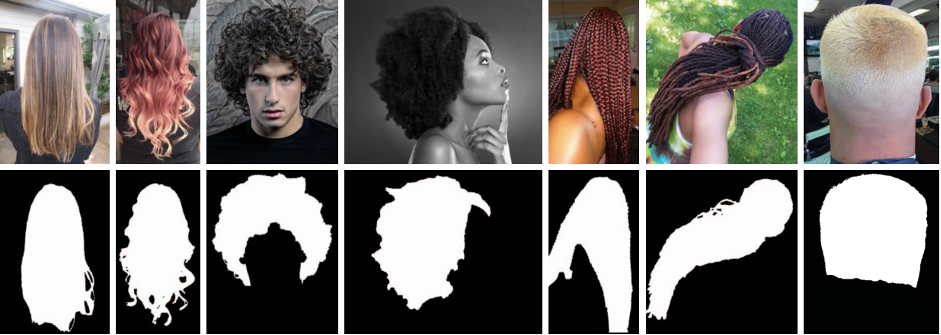
\includegraphics[width=0.9\textwidth]{chapter4/image/figaro.png}
    \caption{Examples of image and mask in Figaro1k dataset}
    \label{fig:figaro}
\end{figure}

Figaro1k consists of 1050 images, equally distributed in seven hairstyle classes. It is regarded as an annotated novel multi-class image database for hair analysis in the wild.

\paragraph{LFW}
LFW,  stands for "Labeled Faces in the Wild", is also an annotated face dataset in the wild dataset. It contains more than 2,000 images of faces collected from the web. Each face has been labeled with the name of the person pictured so that the dataset is also used as the benchmark for the face recognition problem.

\begin{figure} [H]
    \centering
    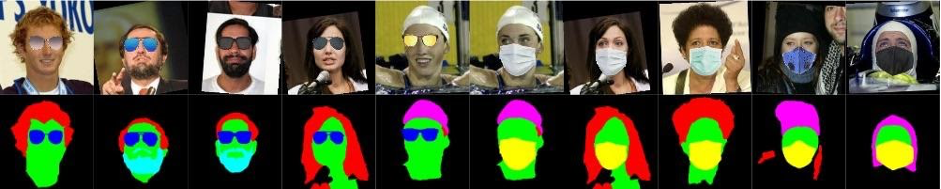
\includegraphics{chapter4/image/lfw.png}
    \caption{Examples of image and mask in LFW dataset}
    \label{fig:lfw}
\end{figure}

Each image is a JPG image with the size of 250x250. The dataset is already split into train, validation, and test set. They have respectively 1500 images, 500 images, and 900 images.
       
\subsection{Data preparation}

In a segmentation task, it is typically challenging to obtain an adequate training set of annotated data. The process of annotation is time-consuming, even when support tools are supplied. However, I used three publicly available datasets: DeepFashion2 for the clothes segmentation task, Figaro1k and LFW for the hair segmentation task. All of them are provided publicly; they have already been attached to annotations. However, they are organized differently. \par

\paragraph{DeepFashion2}
DeepFashion2 is a massive dataset; it has already been divided into the training set, validation set, and test set. The training set has 137.000 images stored in \emph{/image} folder and corresponding annotations located in \emph{/annos} folder, which is adequate for training a deep learning model. However, as the dataset's size is quite big, I read all annotation information and represent them on a Pandas DataFrame. Therefore, the dataset is highly manipulated, and I can easily filter out all data with category\_id bigger than six (because the model only aimed at upper-body clothes recognization). \par

\begin{figure} [H]
    \centering
    \captionsetup{justification=centering}
    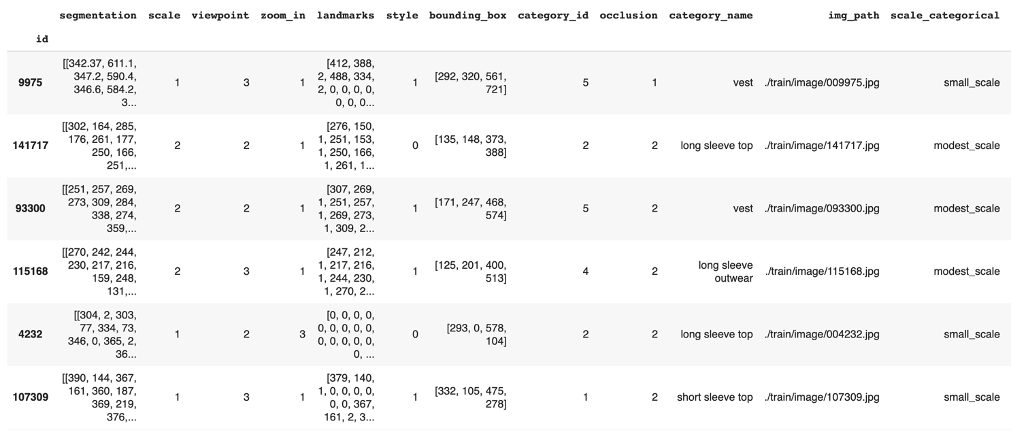
\includegraphics[width=0.9\textwidth]{chapter4/image/dataframe.png}
    \caption{Head of DataFrame of DeepFashion2’s trainning set}
    \label{fig:df}
\end{figure}

The above figure depicts the format of a DataFrame after synthesized from many JSON annotation files. Each row corresponding to an image has information like image path, category, polygons segmentation… \par

\paragraph{Figaro1k and LFW}
Figaro1k and LFW are organized into an image folder and an annotation folder. The image folder consists of images under \emph{jpg} extension, while the annotation folder consists of annotations under the bpm extension. Thus, it is more straightforward to read these two datasets when compared to DeepFashion2. Plus, these two datasets are much more lightweight than DeepFashion2. I use OpenCV2 to encode all images and their corresponding annotations; it outputs a Numpy array, which can forward instantly through the neural network. \par

\subsection{Data augmentation}
Data augmentation is the process of enriching the dataset by applying some transformations to the initial image to generate augmented images. It acts as a regularizer or to speed up convergence, thereby avoid overfitting and improve generalization capabilities. Some image transform operations used in the work are collectively horizontal and vertical flipping, 90-degree rotation, CLAHE, RandomContrast, and RandomGamma. \par

\begin{figure}[H]
    \centering
    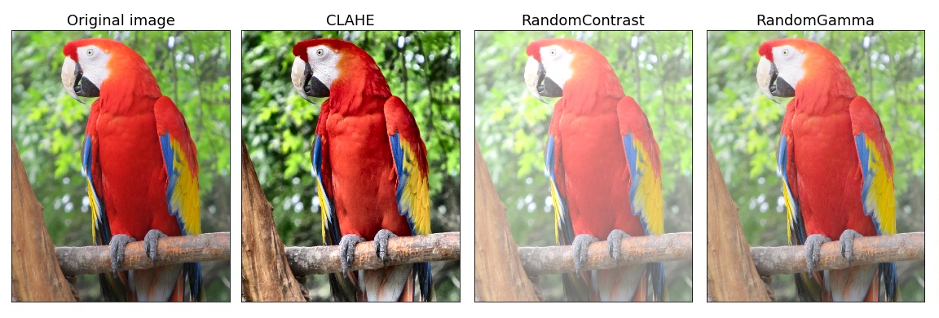
\includegraphics{chapter4/image/augmentation.png}
    \caption{Illustration for transform operations}
    \label{fig:augmentation}
\end{figure}

All of the transformations are composed and applied separately to each image in the dataset with specific probabilities; hence the transformations are guaranteed to apply randomly. As a result, the network sees different data each epoch, and this would generalize the model. \par
I use the Albumentations library \cite{albumentations}, a Python library, to handle the entire augmentation process.


\subsection{Trainning}

The proposed CNN, introduced in \textbf{section \ref{sec:model}}, is implemented by using the Tensorflow framework. The environment used for training is CoLab Pro with 25 GBs of memory, 16 GBs of GPU, and 147 GBs of disk. While the base network load weights pre-trained in the ImageNet dataset, the weights of the rest of the model are initialized randomly.
\par 
The model for hair segmentation is trained in the LFW and Figaro1k dataset with Adam optimization with $\beta_{1} = 0.9$ and $\beta_{2} = 0.999$. The learning rate is set to 1e-3, the batch size is 16. The model is trained for 46 epochs with all parameters trainable.
\par
Meanwhile, the model for clothes segmentation is trained in the DeepFashion2 dataset with Adam optimization with $\beta_{1} = 0.9$ and $\beta_{2} = 0.999$. The learning rate is set to 1e-3, the batch size is 64. The network is trained for 15 epochs. For the first 10 epochs, the base network is frozen. Later, it is unfreezing in the latter 5 epochs.
\par

\section{Results} \label{sec:results}
In this section, I present the result Android app that is developed. The app follows the requirement and use cases which are analyzed in section \textbf{section \ref{sec:usecase}}. At first, I show interfaces of some main activities of the app. After that, the performance of the app is reported. In the second half of this section, I report the accuracy of the hair and clothes segmentation model, which is already proposed in \textbf{section \ref{sec:model}}. 

\subsection{Android app}
\subsubsection{User interface}
An Android app is comprised of one or more activities, meaning one or more screens. Each activity is one screen of that app's user interface. The Android app starts by showing the main activity, and from there, the app may make it possible to open other activities. Here is some core activities of the app:
\begin{itemize}
    \item Main Activity
    \item Color Scanning Activity
    \item Camera Activity
    \item Segmentation Activity
    \item Post-capture Activity
\end{itemize}
The following are screenshots of these activities.

\begin{figure} [H]
    \centering
    \captionsetup{justification=centering}
    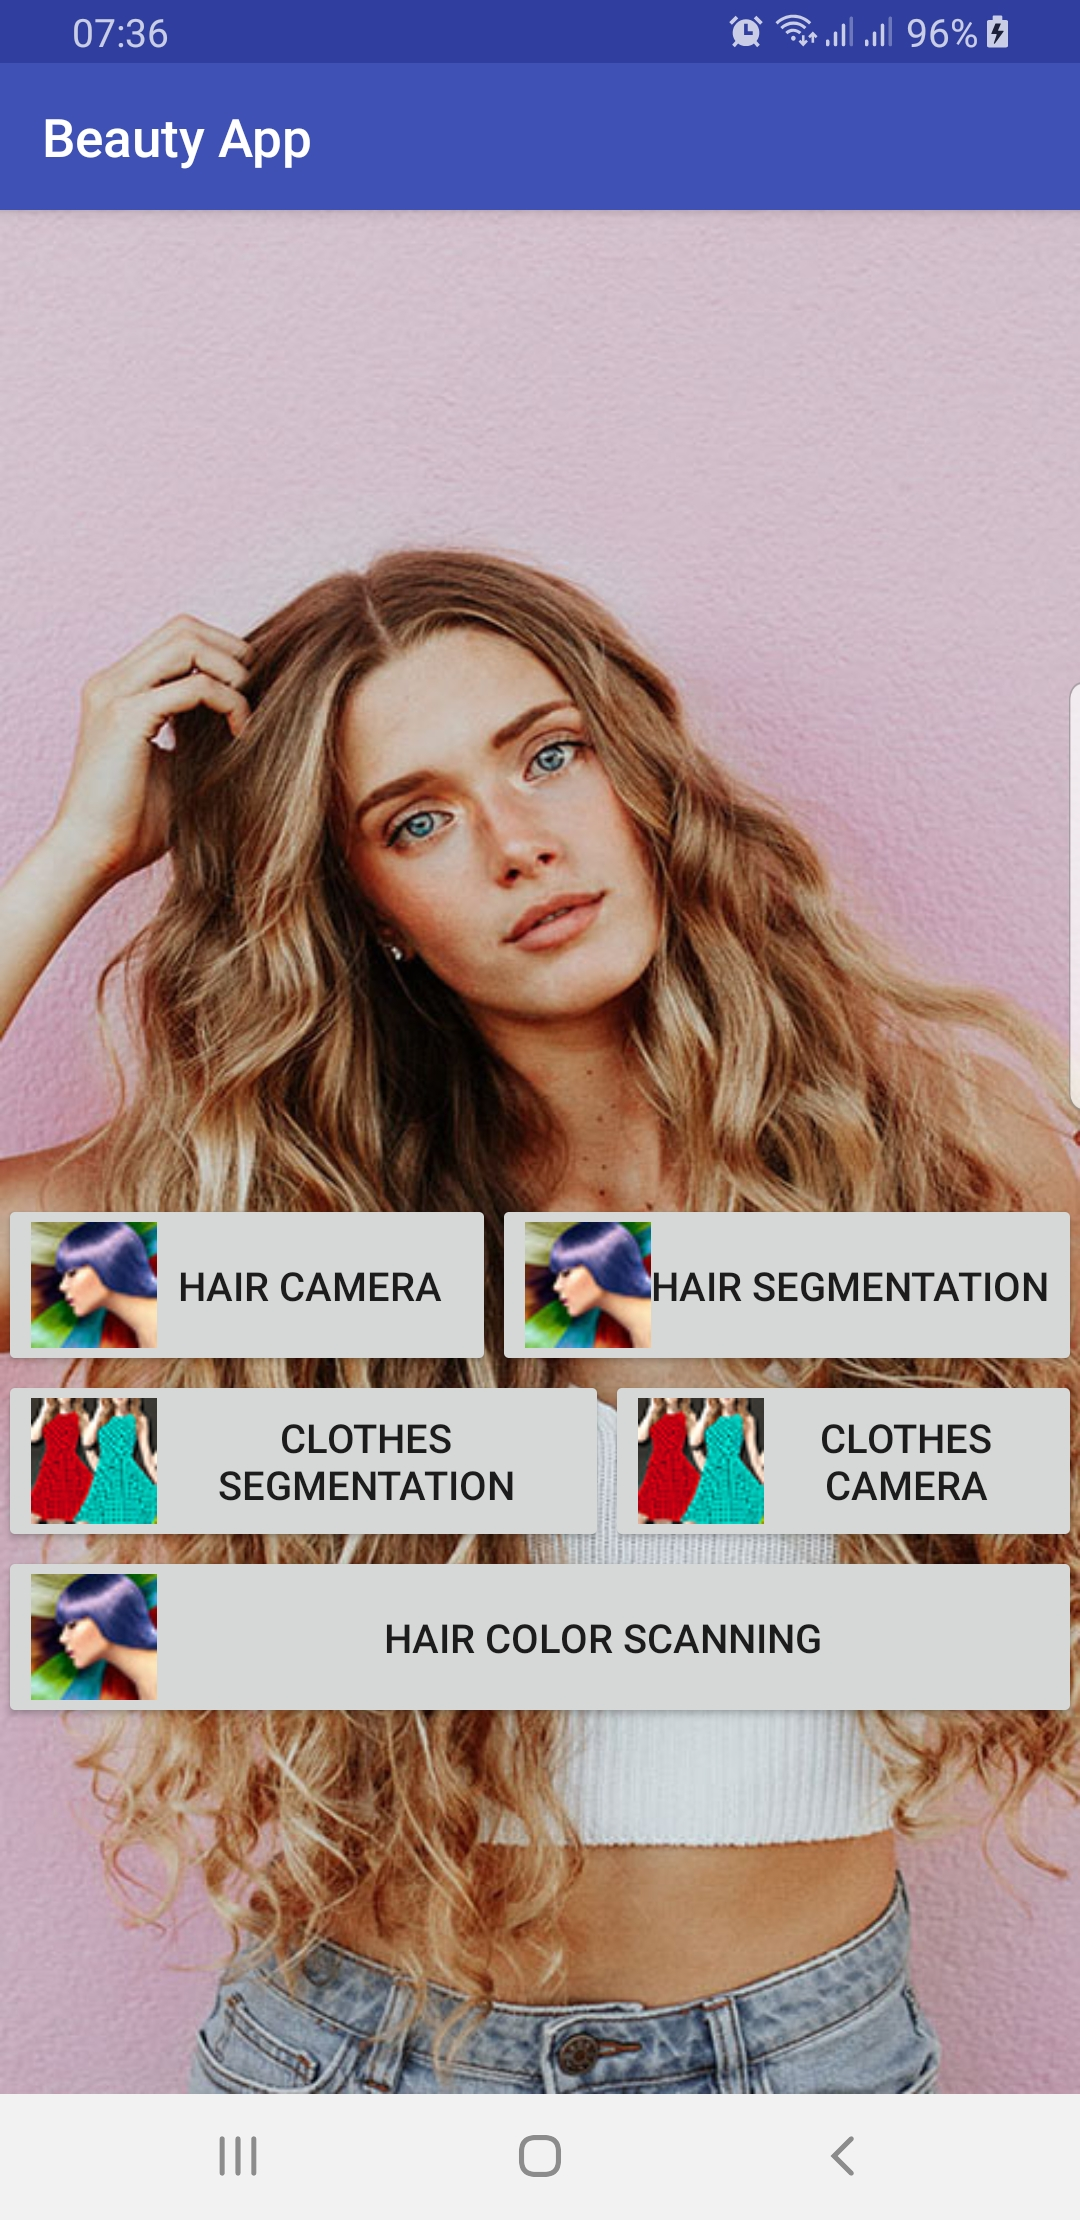
\includegraphics[width=0.3\textwidth]{chapter4/image/home.jpg}
    \caption{Illustration for Main Activity}
\end{figure}

\begin{figure} [H]
    \centering
    \captionsetup{justification=centering}
    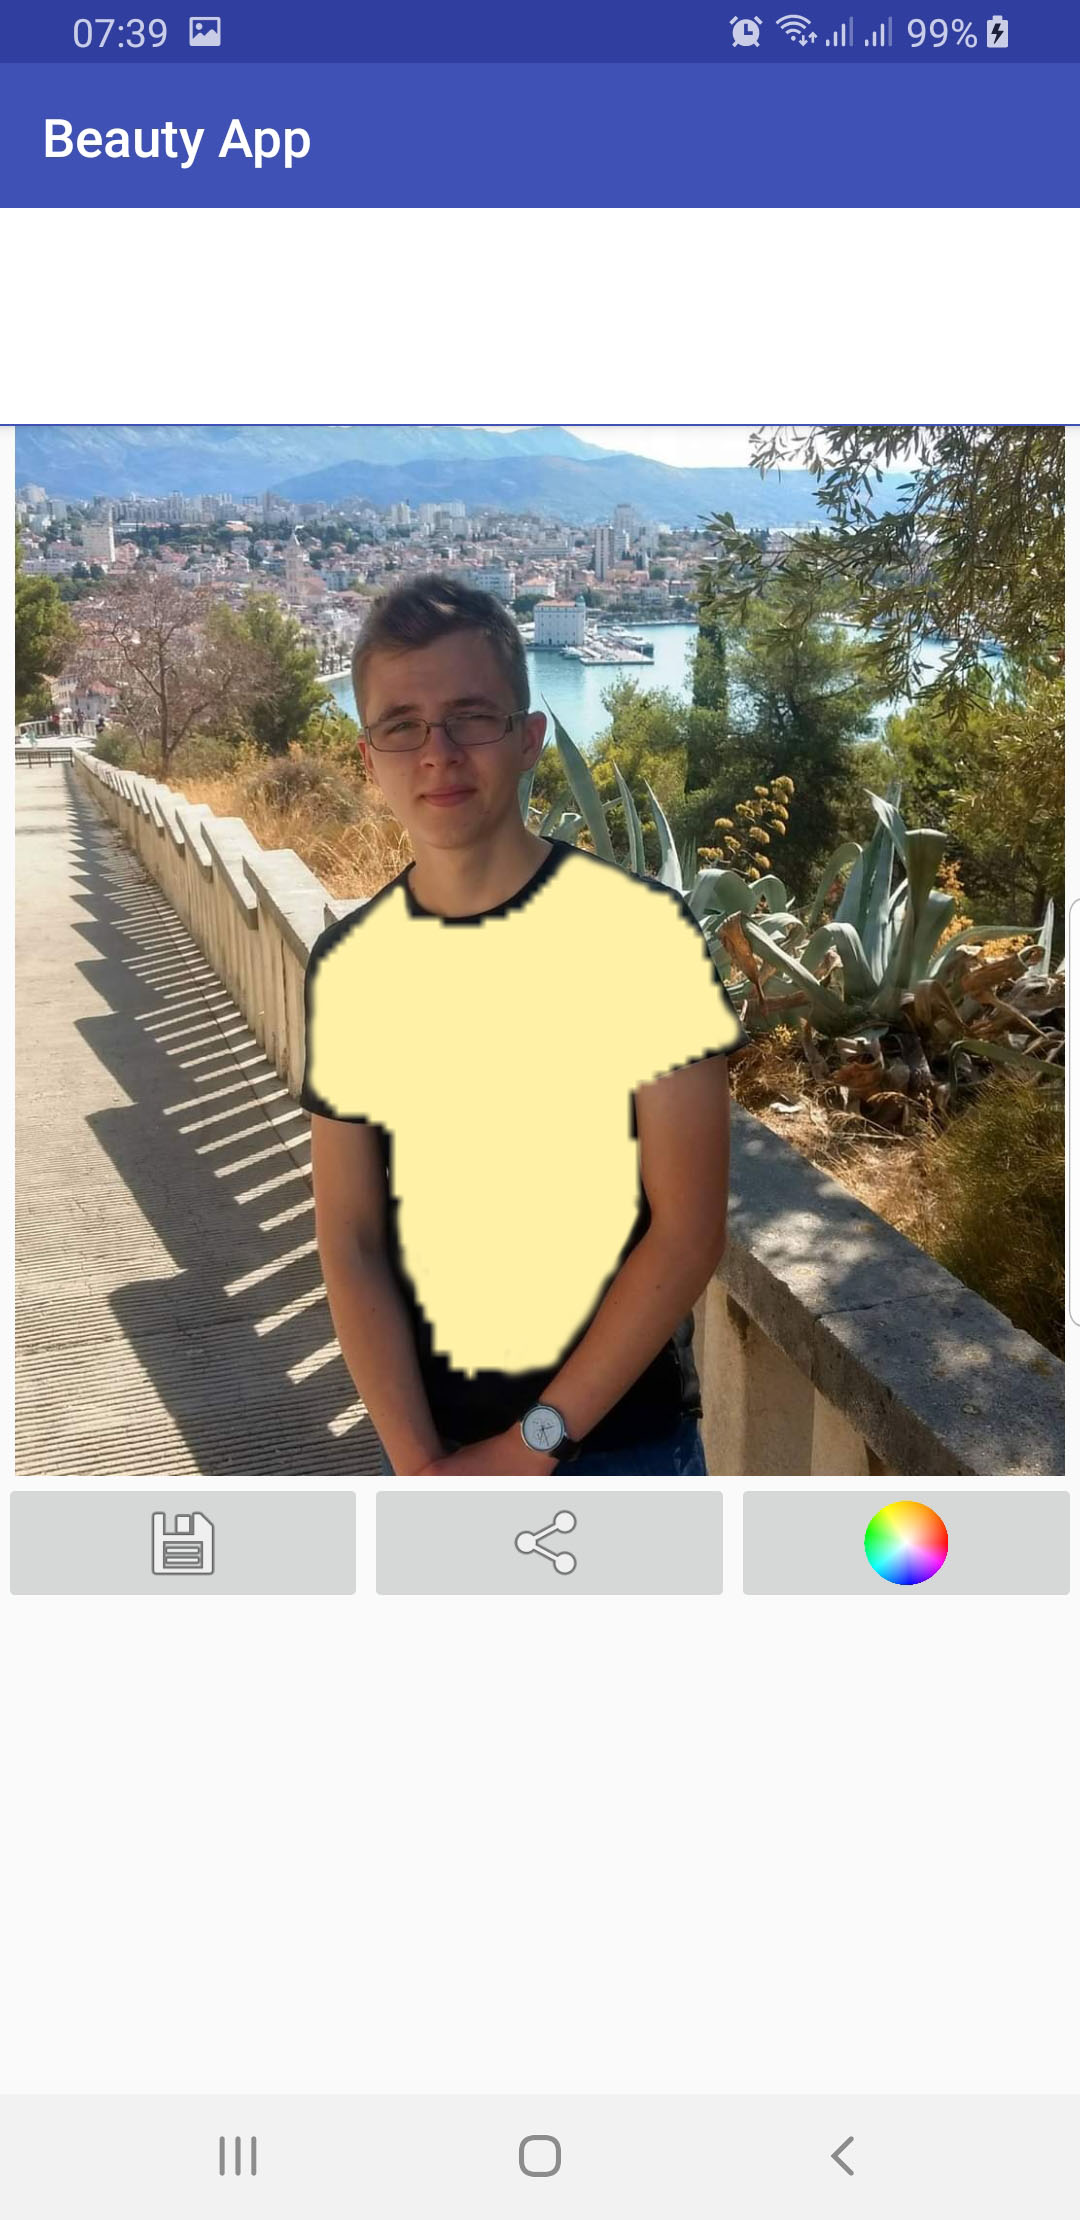
\includegraphics[width=0.3\textwidth]{chapter4/image/segment.jpg}
    \caption{Illustration for Clothes Segmentation Activity}
\end{figure}

\begin{figure} [H]
    \centering
    \captionsetup{justification=centering}
    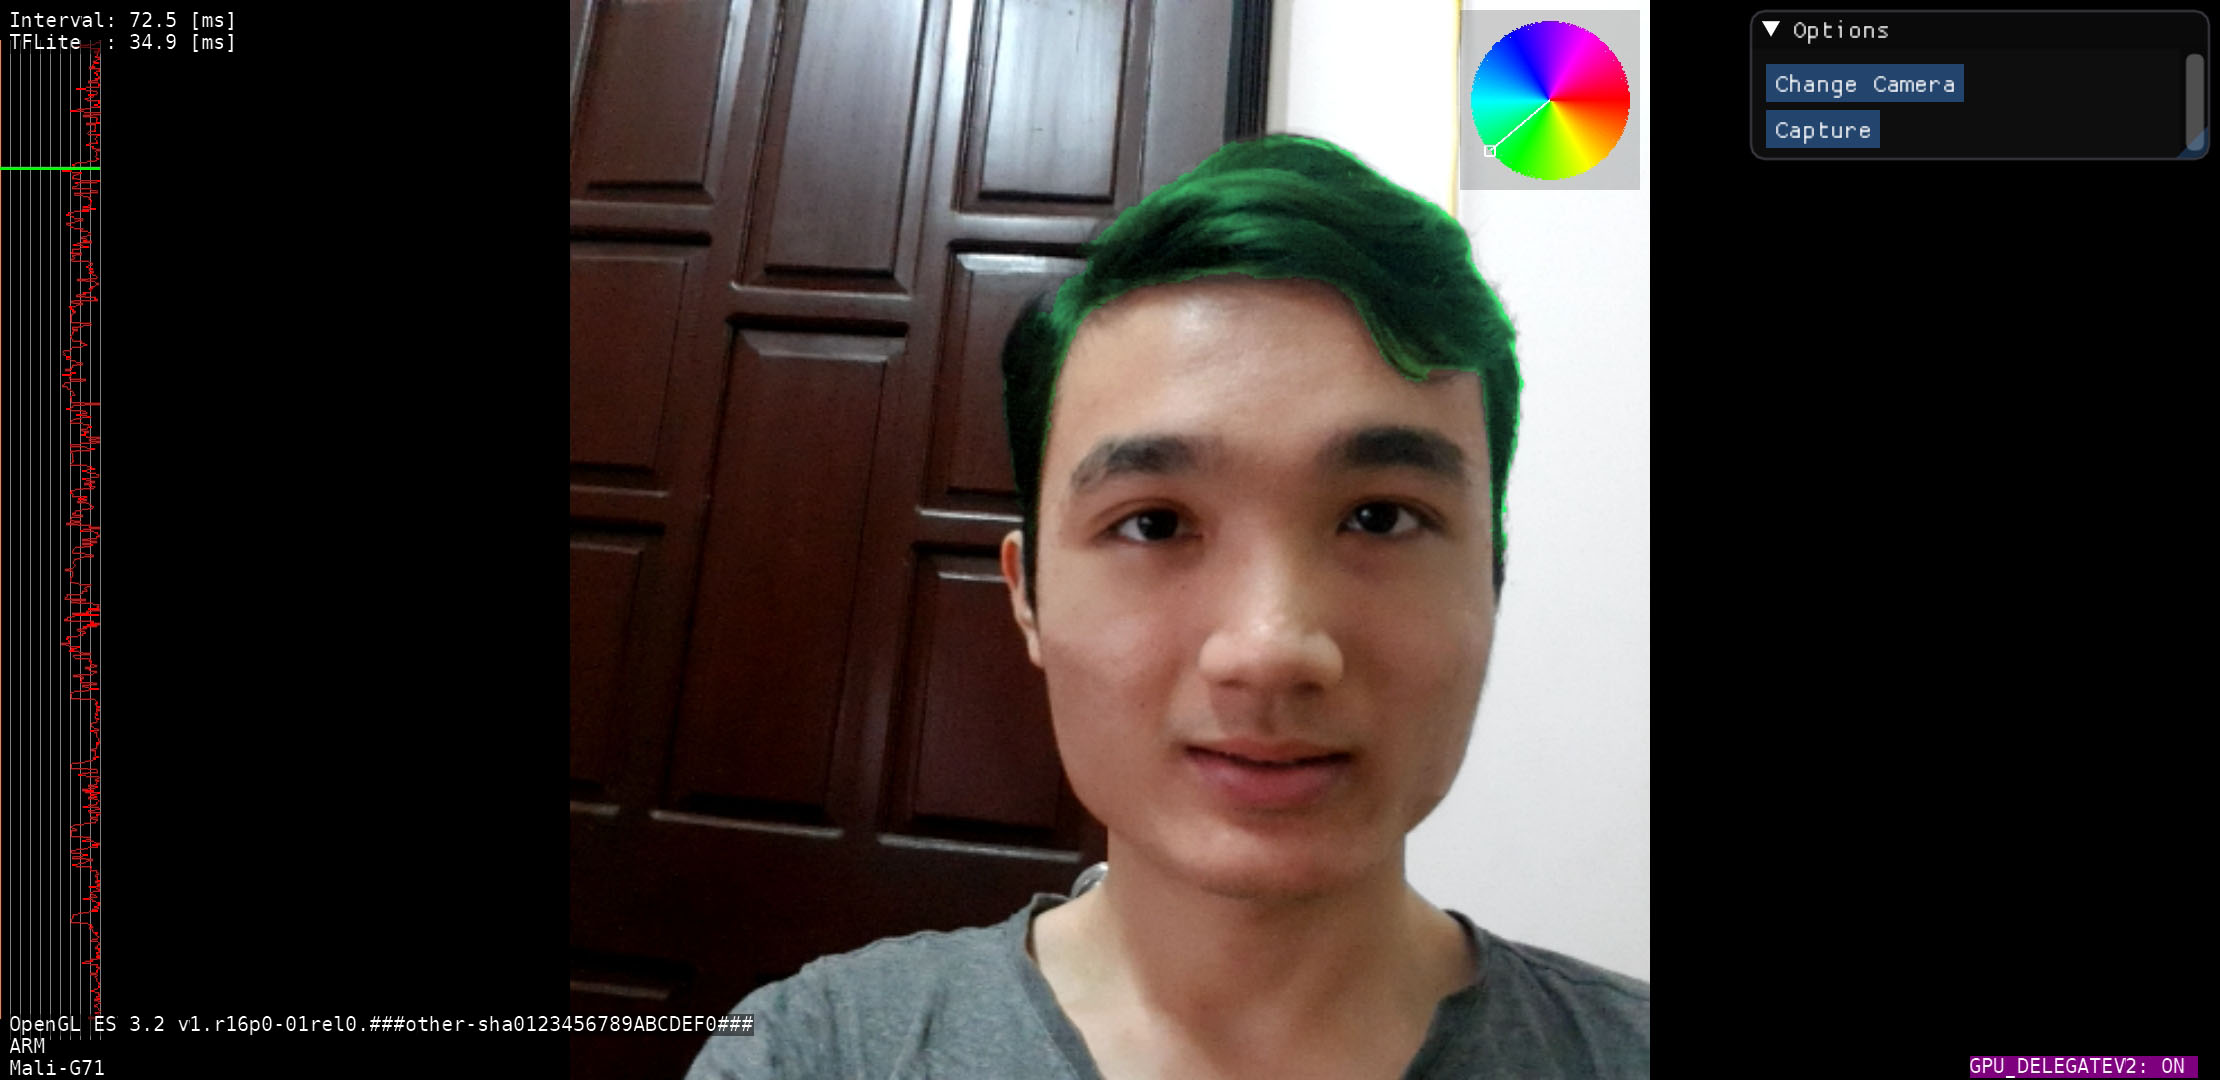
\includegraphics[width=0.7\textwidth]{chapter4/image/scanning.jpg}
    \caption{Illustration for Hair Color Scanning Activity}
\end{figure}


\begin{figure} [H]
    \centering
    \captionsetup{justification=centering}
    
\includegraphics[width=0.3\textwidth]{chapter4/image/camerascreenshot.jpg}
    \caption{Illustration for Clothes Camera Activity}
\end{figure}




\subsubsection{Performance}
Because responsiveness is one of the most important non-functional requirements of the app, the performance is carefully evaluated. It is true that ML apps spend most of their execution time making predictions and rendering these predictions after that. Therefore, I take a measurement of the rendering speed of the two proposed rendering methods, apart from the inference speed of the two proposed models. To do that, I apply methods one by one into a specific use case and collect the results afterward. \par
 
This experiment is conducted on the Samsung S8+, having an ARM Mali-G71 GPU, 4 GBs of memory. The two following tables show the experimental results.

\begin{table}[H]
\centering
\caption{Average inference time of the app} 
 \begin{tabular}{||c c||} 
 \hline
 Model & Inference time (ms) \\ [0.5ex] 
 \hline\hline
  Hair segmentation & 200\\ 
 Cloth segmentation & 240 \\ [1ex] 
 \hline
 \end{tabular}
\end{table}


\begin{table}[H]
\caption{Average rendering speed of the app} 
\centering
 \begin{tabular}{||c c||} 
 \hline
 Method & Rendering time (ms) \\ [0.5ex] 
 \hline\hline
  Bitmap & 43\\ 
 OpenGL & 21 \\ [1ex] 
 \hline
 \end{tabular}
\end{table}


\subsection{Models}

The two proposed models, one for hair and one for clothes, are adapted from the U-Net architecture, already presented in \textbf{section \ref{sec:model}}. The models are trained with the hyperparameters listed in \textbf{section \ref{sec:experiments}}. For hair segmentation models, it is trained for 46 epochs. With the clothes segmentation task, the model is trained for 15 epochs, but in the first 10 epochs, the base net is frozen, in the rest epochs, the base net is unfreezing. All models are tested in the same dataset that they were trained in. The below table shows the results:

\begin{table}[H]
\caption{Accuracy of the proposed models} 
\centering
 \begin{tabular}{||c c||} 
 \hline
 Model & IoU (\%) \\ [0.5ex] 
 \hline\hline
  Hair segmentation & 88\% \\ 
 Clothes segmentation & 84\% \\ [1ex] 
 \hline
 \end{tabular}
\end{table}



\setcounter{figure}{0}
\mychapter{5}{CHAPTER 5. CONCLUSION AND FUTURE WORKS}\label{ch:chap5} 
This chapter concludes the work and then brings out some potential future works. Also, the aim and objectives of the thesis are reviewed, while the achievements are summarised. \par 

\section{Conclusion}

This thesis was conducted to explore how deep learning models can be used for applications requiring artificial intelligence on smartphones and/or other mobile devices. The minority of current deep learning models is compatible with mobile access. Some of such models are mentioned in the second chapter; the reasons why they are not suitable for deployment on mobile devices are listed as well. Moreover, the difficulties in deployment and supplying real-time experience are comprehensively addressed.
 \par
This thesis began with background information and user cases in order to understand the need and purpose of the work. Afterward, a mobile beauty application was designed and developed as a functional prototype for Android mobile phones. Methods for the important issues of the app are analyzed thoroughly and solved besides. Testing and evaluation were also conducted during and at the end of the thesis project by quantitative assessment.
The mobile application includes camera view, real-time recoloring, color scanning. All of them are the crucial features of beauty applications based on the user study. 
Meanwhile, the mobile application is designed to express consistency with the initial requirement from both functionality and user interface point of view. Moreover, as an application running on smartphones, the design and development also considers the limitation of hardware platform, such as computation power, memory size, etc. \par


\section{Future works}

According to the feedback from testing evaluation, a couple of phenomena should be taken care of, and even modified, such as the model optimization for reducing inference time. And more features could be designed and implemented, such as hairstyle transfer.
\par
More importantly, from the deep learning point of view,  an more effective architecture or base network can also be adapted for the work. In terms of frameworks, both Android and Tensorflow have been releasing out many convenient tools for AI developers, lately are metadata and model binding, which can be adapted to the segmentation application. So adapting those addons to this segmentation application is meaningful and effective. \par

Furthermore, the quality of rendering leaves plenty of room for improvement. As we know, the methods of rendering in the thesis are simply to overlay the mask onto the camera view. For that, color transfer applied directly to the camera's images can be potential. 
\par
% \chapter*{Bibliography}
\addcontentsline{toc}{chapter}{Bibliography}

\begin{thebibliography}{9}
\section*{Papers}

\bibitem{hairseg1}
Yongzhe Yan,
\textit{Human Hair Segmentation In The Wild Using Deep Shape Prior}, Computer Vision and Pattern Recognition 2019.

\bibitem{fpn}
Tsung-Yi Lin,
\textit{Feature Pyramid Networks for Object Detection}, Computer Vision and Pattern Recognition 2017.

\bibitem{densenet}
Gao Huang,
\textit{Densely Connected Convolutional Networks}, Computer Vision and Pattern Recognition 2017.

\bibitem{deeplabv3}
Liang-Chieh Chen,
\textit{Rethinking Atrous Convolution for Semantic Image Segmentation}, European Conference on Computer Vision 2018.

\bibitem{deeplabv3plus}
Liang-Chieh Chen,
\textit{Encoder-Decoder with Atrous Separable Convolution for Semantic Image Segmentation}, European Conference on Computer Vision 2018.

\bibitem{pspnet}
H. Zhao,
\textit{Pyramid Scene Parsing Network}, Conference on Computer Vision and Pattern Recognition 2018.

\bibitem{hairseg2matting}
Alex Levinshtein,
\textit{Real-time deep hair matting on mobile devices}, Conference on Computer and Robot Vision 2018.

\bibitem{resnet}
Kaiming He, Xiangyu Zhang, Shaoqing Ren, Jian Sun,
\textit{Deep Residual Learning for Image Recognition},
Computer Vision and Pattern Recognition 2016.

\bibitem{uml}
Ambler, S. W.
\textit{The Elements of UML(TM) 2.0 Style}, Cambridge University Press.

\bibitem{mnasnet}
Mingxing Tan,
\textit{MnasNet: Platform-Aware Neural Architecture Search for Mobile}, Conference on Computer and Robot Vision 2019.

\bibitem{mobiledets}
Yunyang Xiong,
\textit{MobileDets: Searching for Object Detection Architectures for Mobile
Accelerators}, Conference on Computer and Robot Vision 2021.

\bibitem{maskrcnn}
Kaiming He,
\textit{Mask R-CNN}, International Conference on Computer Vision 2017.

\bibitem{albumentations}
A. Buslaev,
\textit{Albumentations: fast and flexible image augmentations}, arXiv:1809.06839.

\bibitem{carbonemission}
WRAP,
\textit{Valuing Our Clothes}, The Cost of UK Fashion 2017.


\bibitem{deepfashion2}
Yuying Ge,
\textit{DeepFashion2: A Versatile Benchmark for Detection, Pose Estimation, Segmentation and Re-Identification of Clothing Images}, 
Computer Vision and Pattern Recognition 2019.

\bibitem{unet}
O. Ronneberger, P. Fischer, T. Brox,
\textit{U-Net: Convolutional Networks for Biomedical Image Segmentation}, 
International Conference on Medical Image Computing and Computer-Assisted Intervention 2015.


\bibitem{squeezenet}
Forrest N. Iandola,
\textit{U-Net: Convolutional Networks for Biomedical Image Segmentation}, 
International Conference on Medical Image Computing and Computer-Assisted Intervention 2015.


\bibitem{mnasnet}
M. Tan, B. Chen, R. Pang, V. Vasudevan,
\textit{Mnasnet: Platform-aware neural architecture search for mobile}, Computer Vision and Pattern Recognition 2019.

\bibitem{mobilenetv1}
AG. Howard, M. Zhu, B. Chen, D. Kalenichenko,
\textit{MobileNets: Efficient Convolutional Neural Networks for Mobile Vision Applications}, Computer Vision and Pattern Recognition 2019.


\bibitem{mobilenetv2}
Mark Sandler,
\textit{MobileNetV2: Inverted Residuals and Linear Bottlenecks}, arXiv:1704.04861.

\bibitem{openglpipeline}
S. Türkmen,
\textit{Scene Understanding Through Semantic Image Segmentation in Augmented Reality}, urn.fi/URN:NBN:fi:oulu-201906262666.

\bibitem{segnet}
Vijay Badrinarayanan,
\textit{SegNet: A Deep Convolutional Encoder-Decoder Architecture for Image Segmentation}, arXiv:1511.00561.

\bibitem{vgg}
Karen Simonyan, Andrew Zisserman,
\textit{Very Deep Convolutional Networks for Large-Scale Image Recognition}, 	arXiv:1409.1556.

\bibitem{thundernet}
Zheng Qin,
\textit{ThunderNet: Towards Real-time Generic Object Detection}, 		arXiv:1903.11752.

\section*{Websites}

\bibitem{jetpack}
https://developer.android.com/jetpack

\bibitem{qnnpack}
https://engineering.fb.com/2018/10/29/ml-applications/qnnpack/

\bibitem{androiddev}
https://developer.android.com/guide/topics/graphics/opengl

\bibitem{cs231n}
http://cs231n.github.io/neural-networks-1/

\bibitem{platformprediction}
https://cloud.google.com/ai-platform/prediction/docs

\bibitem{cloudfunctions}
https://cloud.google.com/blog/products/ai-machine-learning/how-to-serve-deep-learning-models-using-tensorflow-2-0-with-cloud-functions

\bibitem{googlecloudml}
https://cloud.google.com/ai-platform

\bibitem{tfserving}
https://github.com/tensorflow/serving




\end{thebibliography}

\end{document}
    